\subsection[SU(p,q)]{$\mathrm{SU}(p,q), p+q=n \sim A_{n-1}, n \geq 2$}\label{sec:su}

\subsubsection{Root system data}

\[\alpha_i = \epsilon_i - \epsilon_{i+1}, \quad \omega_i = \epsilon_1 + \cdots + \epsilon_i \]
\begin{align*}
 \roots & = \{ \epsilon_i - \epsilon_j | i\neq j, i,j=1\ldots n\}\\
 \roots_c^+ & = \{ \epsilon_i-\epsilon_j | 1\leq i < j \leq p \text{ or } p+1 \leq i < j \leq n\}\\
 \roots_n^+ & = \{ \epsilon_i - \epsilon_j | 1 \leq i \leq p, p+1 \leq j \leq n \}
\end{align*}
\[\beta = \epsilon_1 - \epsilon_n,\quad 2\rho = (n-1,n-3,\ldots -n+3,-n+1),\quad \zeta = (\underbrace{\frac{q}{n},\ldots,\frac{q}{n}}_{p\text{ times}},\underbrace{\frac{-p}{n},\ldots,\frac{-p}{n}}_{q\text{ times}})\]
\inserttikzfigure{diagrams/dynkin_An_p.tikz}{Marked Dynkin diagram of $\lie{su}(p,q)$ for $p+q=n$}

The reduction points of unitarizable highest weight modules are the following integral translated cones $\lambda_a + C_a$:
Let $a=(Q,R,l)$, $Q=R=\mathrm{SU}(p',q')$, $1\leq p' \leq p$, $1\leq q'\leq q$. Then
\[
 C_a = \{a_{p'}\omega_{p'} + \cdots + a_p\omega_p + \cdots + a_{n-q'}\omega_{n-q'} \,|\, a_p=-a_{p'}-\cdots -a_{p-1}-a_{p+1} - \cdots - a_{n-q'} \}.
\]
\begin{gather*}
  \lambda_a=\omega_{p'} + \omega_{n-q'} - (n+l+1-p'-q')\omega_p   \\
  \mu_a = \omega_{p'-l}+\omega_{n-q'+l}-(n+l+1-p'-q')\omega_p\\
  1\leq p' \leq p,\quad 1\leq q' \leq q,\quad 1\leq l \leq \min(p',q')\\
  Q(\lambda_a)=R(\lambda_a)=\mathrm{SU}(p',q')
\end{gather*}

\subsubsection{Nilpotent cohomology in detail}
Now we compute the cohomology for $\lambda = \omega_{p'} + \omega_{n-q'} - (n+l+1-p'-q')\omega_p$. We have for $k=2-(n+l+1-p'-q') = 1+p'+q'-n-l$ that
 \[
  (\epsilon_i, \lambda) = \begin{cases}
                           k, &1\leq i \leq p' \\
                           k-1, & p' < i \leq p\\
                           1, & p < i \leq n-q'\\
                           0, & n-q' < i \leq n.
                          \end{cases}
 \]
 The positive roots of $\lie{su}(p,q)$ are $\epsilon_i - \epsilon_j$, $i<j$ and we have
 \[(\epsilon_i - \epsilon_j, \rho) =  \frac{n+1-2i}{2}-\frac{n+1-2j}{2} = j-i > 0.\] Now, in order to determine the set $\Psi^+_\lambda$, we compute all possible values of $(\epsilon_i - \epsilon_j, \lambda +\rho)$  for $i<j$
 \begin{center}
 \begin{tabular}{C|CCCC}
                  & 1\leq j \leq p' & p' < j \leq p &  p < j \leq n-q' &  n-q' < j \leq n \\[2pt]\hline
  1\leq i \leq p' &         j-i     &    1 + j-i    &      k-1 + j-i   &       k + j-i          \\
  p' < i \leq p   &                 &        j-i    &      k-2 + j-i   &       k-1 + j-i          \\
  p < i \leq n-q' &                 &               &         j-i      &       1 + j-i          \\
  n-q' < i \leq n &                 &               &                  &       j-i          \\
\end{tabular}
\end{center}
We see that only terms containing $k$ can be zero, because $j-i >0$ and $2-n \leq k \leq 0$. Thus the only singular roots are the noncompact ones. Substituting for $k$ and solving for $j$ we get
% \begin{center}
% \begin{tabular}{C|CC}
%  &  p < j \leq n-q' &  n-q' < j \leq n \\[2pt]\hline
%    1\leq i \leq p' &            p'+q'-n-l + j-i   &       1+p'+q'-n-l + j-i          \\
%   p' < i \leq p   &    -1+p'+q'-n-l + j-i   &       p'+q'-n-l + j-i          \\
% \end{tabular}
% \end{center}
% and solving for zero
\begin{center}
\begin{tabular}{C|CC}
                   &  p < j \leq n-q'    &  n-q' < j \leq n \\[2pt]\hline
   1\leq i \leq p' &  j=i+m   &   j=i+m-1         \\
  p' < i \leq p    &  j=i+m+1 &   j=i+m       \\
\end{tabular}
\end{center}
where \[m=1-k = n+l-p'-q'.\]
The case $j=i+m+1$ doesn't lead to any solution, since $j-i-m-1 = j-i-n-l+p'+q'-1$ is strictly negative for $ p' < i \leq p < j \leq n-q' $.
%for $i=p'+1$ we get $j=2+l+n-q'>n-q'$.
The case $j=i+m$ for $i \leq p'$ leads to
\begin{gather*}
 \max\{1,q'-q+1+p'-l\}\leq i \leq p'-l\\
 \max\{1+n+l-p'-q', p+1 \} \leq j \leq n-q',
\end{gather*}
which results in an empty set of singular roots if and only if $l=p'$.
The case of $j=i+m$ for $i>p'$ yields
\begin{gather*}
  p'+1 \leq i \leq \min\{p, p'+q'-l \}\\
  n-q'+l+1 \leq j \leq \min\{n +l-p'-q'+p,n \},
\end{gather*}
which gives an empty set of singular roots if and only if $l=q'$ or $p=p'$.
And finally the case $j=i+m-1$ gives
\begin{gather*}
 p'+2-l \leq i \leq p'\\
 n-q'+1 \leq j \leq n-q'-1+l
\end{gather*}
which doesn't contribute to singular roots if and only if $l=1$.

Two roots $\epsilon_i - \epsilon_j$, $\epsilon_a - \epsilon_b$ are orthogonal if and only if $\{i,j\} \cap \{a,b\}=\emptyset$. Thus the set of positive noncompact roots orthogonal to $\Psi_\lambda^+$ is
\begin{multline}\label{eq:orthogonal_to_singular}
\big\{\epsilon_i - \epsilon_j\,|\,
		i \in \{ 1,\ldots, q'-q+p'-l\}\cup \{p'-l+1\}\cup \{ p'+q'-l+1,\ldots, p \} \\
		j \in \{p+1,\ldots,  m\} \cup \{n+l-q'\} \cup \{m+p+1, \ldots,n\} \big\},
% 		j \in \{p+1,\ldots,  n+l-p'-q'-1\} \cup \{n+l-q'\} \cup \{n+l-p'-q'+p+1, \ldots,n\} \big\}.
\end{multline}
where a set $\{a,\ldots,b\}$ is considered empty if $a>b$.

Positive noncompact roots $\alpha = \epsilon_i - \epsilon_j$ satisfying $(\lambda + \rho, \alpha)\in \Z^+$ are given by constraints
\begin{equation}\label{eq:su_root_constraints}
\begin{split}
 1 \leq i \leq p' & \Longrightarrow \max \{ i+m, p \} < j \leq n-q' \vee \max \{ i+m, n-q'+1 \}  \leq j \leq n  \\
 p' < i \leq p & \Longrightarrow \max \{p, i+m+1 \} < j \leq n-q' \vee \max \{n-q',i+m\} < j  \leq n.
 \end{split}
\end{equation}

If a positive noncompact root $\epsilon_i - \epsilon_j$ with $i>p'$ is orthogonal to all singular roots and it's scalar product with $\lambda + \rho$ is positive, then necessarily
\[
 i\in \{ p'+q'-l+1,\ldots, p \} \text{ and } i+m < j\leq n.
\]
But for $i=p'+q'-l+1$ we get that $i+m = n+1$ and hence we see that there are no such roots. Thus, we have to look only at the noncompact roots satisfying the first constraint of \eqref{eq:su_root_constraints}.

If a noncompact root $\epsilon_i - \epsilon_j$ with $i\leq p'$ is orthogonal to the singular roots $\Psi_\lambda^+$, then either $i=p'-l+1$ or $i \leq q'-q + p'-l$. If $i=p'-l+1$, then we get $i+m = n-q'+1$ which means that we have to look only at
\[
 \max \{ i+m, n-q'+1 \} = n-q'+1  \leq j \leq n.
\]
Taking into account \eqref{eq:orthogonal_to_singular} we see that the roots with indices given by
\[
 i = p'-l+1, \quad j \in \{n-q'+l\} \cup \{m+p+1, \ldots,n\}
\]
are included in $\roots_{n,\lambda}^+$. For  $i\leq q'-q + p'-l$ we have $i+m \leq p$ and the constraints of \eqref{eq:su_root_constraints} reduce to
\[
 p < j \leq n
\]
and thus the remaining roots of $\roots_{n,\lambda}^+$ have indices given by
\[
  i \in \{ 1,\ldots, q'-q+p'-l\}, \quad
  j \in \{p+1,\ldots,  m\} \cup \{n+l-q'\} \cup \{m+p+1, \ldots,n\}.
\]

Because all roots have the same length $\sqrt{2}$ we finally arrive at $\roots_{n,\lambda}^+ $ being equal to the set of roots $\epsilon_i - \epsilon_j$ with indices given by the following constraints
\begin{gather}
  i = p'-l+1 \quad \&\quad  j \in \{n-q'+l\} \cup \{m+p+1, \ldots,n\} \\ \notag
  i \in \{ 1,\ldots, q'-q+p'-l\} \quad \& \hspace{8cm} \\ \notag \hspace{4.5cm}  j \in \{p+1,\ldots,  m\} \cup \{n+l-q'\} \cup \{m+p+1, \ldots,n\}.\notag
\end{gather}

The Weyl group of $\lie{sl}(n)$ is generated by root reflections and is isomorphic to the symmetric group $S_n$ on the set $\{1,\ldots,n\}$. Indeed, the reflection $s_{\epsilon_i - \epsilon_j}$ acts as a transposition of the $i$th and $j$th coordinate in $\epsilon$-basis. Since there are overlaps in the ranges for $j$ for various $i$, it follows that the group $W_\lambda$ is isomorphic to the permutation subgroup of $S_n$ which permutes only a subset $M_\lambda$ of $\{1,\ldots,n\}$ and leaves all other elements fixed. This subset is
\[
 M_\lambda =  \{ 1,\ldots, q'-q+p'-l, p'-l+1, p+1,\ldots,m, n-q'+l,m+p+1,\ldots,n\}
\]
in the case of $q'-q+p'-l > 0$ and
\[
  M_\lambda =  \{p'-l+1,n-q'+l,m+p+1,\ldots,n\}
\]
if $q'-q+p'-l \leq 0.$ We remind, that a range $a,\ldots,b$ is considered empty if $a>b$. The root subsystem $\roots_\lambda$ is then given by
\[
 \roots_\lambda = \{ \epsilon_i - \epsilon_j \,|\, i\neq j, i,j\in M_\lambda \}.
\]

The pair $(\roots_\lambda,\roots_{\lambda,c})$ is a pair of root systems such that the corresponding Lie algebras $(\lie{g}_\lambda,\lie{g}_{\lambda,c})$ form a Hermitian symmetric pair of type $\lie{su}(a,b)$ for some $a,b$. The formula of the theorem \ref{thm:cohomology} is basically coming (via Enright Shelton equivalences) from the classical Kostant formula for Lie algebra cohomology of the nilradical coming from $\lie{g}_\lambda$. Hence the cohomology groups can be computed in a classical way just by restriction to the indices contained in $M_\lambda$.

Let us look at some specific cases. For $p=1$ the only possible value for $l$ is $1$ and $1\leq q' \leq n-1$. The weights are $\lambda = (q'-n)\omega_1 + \omega_{n-q'}$ and the corresponding set $M_\lambda = \{ 1,n-q'+1,\ldots,n \}$.


Now let's look what happens when $p=2$. There are three possibilities
\begin{enumerate}
 \item $p'=1, l=1$\\
 The weight is $\lambda=\omega_1+\omega_{n-q'}-(n+1-q')\omega_2$ and the resulting set of admissible indices $M_\lambda = \{1,n-q'+1,\ldots,n\}$.
 \item $p'=2, l=1$\\
 The weight is $\lambda=\omega_2+\omega_{n-q'}-(n-q')\omega_2 = \omega_{n-q'} + (q'-n+1)\omega_2$ and the resulting set of admissible indices $M_\lambda = \{1,\ldots,n\}$ if $q'=q$ (in which case $\lambda = 0$) and $M_\lambda = \{2,n-q'+1,\ldots,n\}$ for $q'<q$.
 \item $p'=2, l=2$\\
 The weight is $\lambda=\omega_2+\omega_{n-q'}-(n+1-q')\omega_2 = \omega_{n-q'}+(q'-n)\omega_2$ and the resulting set of admissible indices $M_\lambda = \{1,n-q'+2,\ldots,n\}$.
\end{enumerate}

The most singular case occurs for $\lie{su}(k,k)$ and $p'=q'=l = k $. Then the set $M_\lambda =$ is $\{1,2k\}$. For $p'=q'=k$ and $l<k$ we get $M_\lambda = \{ 1,\ldots,k-l+1,k+l,\ldots, 2k \}$.

\subsubsection*{Examples of posets of minimal length representatives}

\begin{figure}[H]
  \centering 
  \begin{tikzpicture}[>=latex,line join=bevel,]
%%
\node (alpha1+alpha2+alpha3+alpha4+alpha5) at (55bp,7bp) [draw,draw=none] {$\alpha_{1} + \alpha_{2} + \alpha_{3} + \alpha_{4} + \alpha_{5}$};
  \node (alpha1) at (55bp,206bp) [draw,draw=none] {$\alpha_{1}$};
  \node (alpha1+alpha2+alpha3+alpha4) at (55bp,57bp) [draw,draw=none] {$\alpha_{1} + \alpha_{2} + \alpha_{3} + \alpha_{4}$};
  \node (alpha1+alpha2+alpha3) at (55bp,107bp) [draw,draw=none] {$\alpha_{1} + \alpha_{2} + \alpha_{3}$};
  \node (alpha1+alpha2) at (55bp,157bp) [draw,draw=none] {$\alpha_{1} + \alpha_{2}$};
  \draw [black,->] (alpha1) ..controls (55bp,193.84bp) and (55bp,183.19bp)  .. (alpha1+alpha2);
  \draw [black,->] (alpha1+alpha2) ..controls (55bp,143.29bp) and (55bp,133.02bp)  .. (alpha1+alpha2+alpha3);
  \draw [black,->] (alpha1+alpha2+alpha3+alpha4) ..controls (55bp,43.293bp) and (55bp,33.024bp)  .. (alpha1+alpha2+alpha3+alpha4+alpha5);
  \draw [black,->] (alpha1+alpha2+alpha3) ..controls (55bp,93.293bp) and (55bp,83.024bp)  .. (alpha1+alpha2+alpha3+alpha4);
%
\end{tikzpicture} 
	\begin{tikzpicture}[>=latex,line join=bevel,]
%%
\node (s1) at (26bp,198bp) [draw,draw=none] {$s_{1}$};
  \node (1) at (26bp,247bp) [draw,draw=none] {$1$};
  \node (s1*s2*s3) at (26bp,102bp) [draw,draw=none] {$s_{1}s_{2}s_{3}$};
  \node (s1*s2) at (26bp,150bp) [draw,draw=none] {$s_{1}s_{2}$};
  \node (s1*s2*s3*s4*s5) at (26bp,6bp) [draw,draw=none] {$s_{1}s_{2}s_{3}s_{4}s_{5}$};
  \node (s1*s2*s3*s4) at (26bp,54bp) [draw,draw=none] {$s_{1}s_{2}s_{3}s_{4}$};
  \draw [black,->] (s1) ..controls (26bp,185.55bp) and (26bp,175.07bp)  .. (s1*s2);
  \draw [black,->] (s1*s2*s3) ..controls (26bp,89.554bp) and (26bp,79.067bp)  .. (s1*s2*s3*s4);
  \draw [black,->] (s1*s2*s3*s4) ..controls (26bp,41.554bp) and (26bp,31.067bp)  .. (s1*s2*s3*s4*s5);
  \draw [black,->] (1) ..controls (26bp,233.83bp) and (26bp,223.21bp)  .. (s1);
  \draw [black,->] (s1*s2) ..controls (26bp,137.55bp) and (26bp,127.07bp)  .. (s1*s2*s3);
%
\end{tikzpicture} 
  \caption{Poset of noncompact roots and the Bruhat graph for $\mathrm{SU}(1,5)$}
\end{figure} 

\begin{figure}[H]
  \centering 
  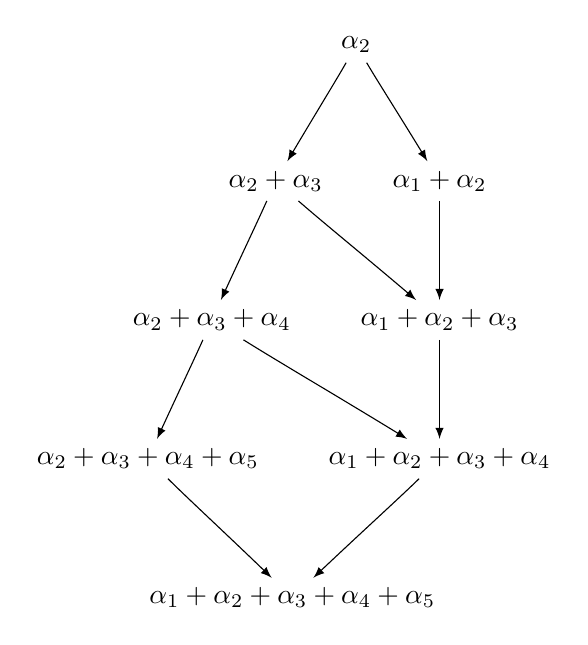
\begin{tikzpicture}[>=latex,line join=bevel,]
%%
\node (alpha2) at (118bp,206bp) [draw,draw=none] {$\alpha_{2}$};
  \node (alpha2+alpha3+alpha4+alpha5) at (43bp,57bp) [draw,draw=none] {$\alpha_{2} + \alpha_{3} + \alpha_{4} + \alpha_{5}$};
  \node (alpha2+alpha3+alpha4) at (66bp,107bp) [draw,draw=none] {$\alpha_{2} + \alpha_{3} + \alpha_{4}$};
  \node (alpha1+alpha2+alpha3+alpha4) at (148bp,57bp) [draw,draw=none] {$\alpha_{1} + \alpha_{2} + \alpha_{3} + \alpha_{4}$};
  \node (alpha1+alpha2) at (148bp,157bp) [draw,draw=none] {$\alpha_{1} + \alpha_{2}$};
  \node (alpha2+alpha3) at (89bp,157bp) [draw,draw=none] {$\alpha_{2} + \alpha_{3}$};
  \node (alpha1+alpha2+alpha3) at (148bp,107bp) [draw,draw=none] {$\alpha_{1} + \alpha_{2} + \alpha_{3}$};
  \node (alpha1+alpha2+alpha3+alpha4+alpha5) at (95bp,7bp) [draw,draw=none] {$\alpha_{1} + \alpha_{2} + \alpha_{3} + \alpha_{4} + \alpha_{5}$};
  \draw [black,->] (alpha2+alpha3+alpha4+alpha5) ..controls (57.627bp,42.498bp) and (70.704bp,30.428bp)  .. (alpha1+alpha2+alpha3+alpha4+alpha5);
  \draw [black,->] (alpha2) ..controls (125.34bp,193.5bp) and (132.69bp,181.99bp)  .. (alpha1+alpha2);
  \draw [black,->] (alpha1+alpha2+alpha3+alpha4) ..controls (133.01bp,42.426bp) and (119.5bp,30.186bp)  .. (alpha1+alpha2+alpha3+alpha4+alpha5);
  \draw [black,->] (alpha2) ..controls (110.91bp,193.5bp) and (103.8bp,181.99bp)  .. (alpha2+alpha3);
  \draw [black,->] (alpha2+alpha3) ..controls (105.77bp,142.35bp) and (121.03bp,129.94bp)  .. (alpha1+alpha2+alpha3);
  \draw [black,->] (alpha2+alpha3) ..controls (82.807bp,143.08bp) and (77.657bp,132.33bp)  .. (alpha2+alpha3+alpha4);
  \draw [black,->] (alpha2+alpha3+alpha4) ..controls (89.571bp,92.203bp) and (112.57bp,78.739bp)  .. (alpha1+alpha2+alpha3+alpha4);
  \draw [black,->] (alpha1+alpha2+alpha3) ..controls (148bp,93.293bp) and (148bp,83.024bp)  .. (alpha1+alpha2+alpha3+alpha4);
  \draw [black,->] (alpha1+alpha2) ..controls (148bp,143.29bp) and (148bp,133.02bp)  .. (alpha1+alpha2+alpha3);
  \draw [black,->] (alpha2+alpha3+alpha4) ..controls (59.807bp,93.076bp) and (54.657bp,82.328bp)  .. (alpha2+alpha3+alpha4+alpha5);
%
\end{tikzpicture} 
	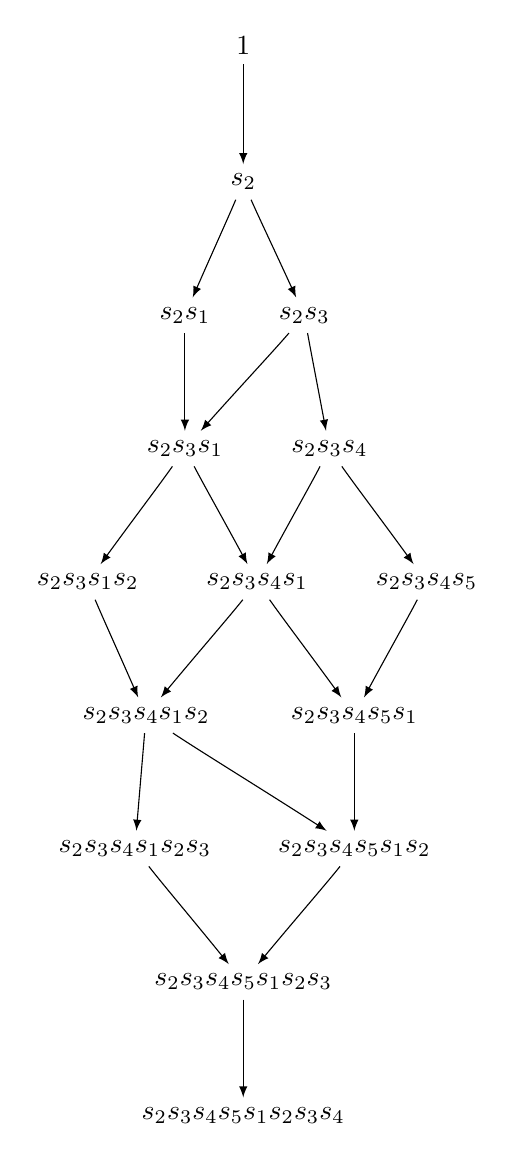
\begin{tikzpicture}[>=latex,line join=bevel,]
%%
\node (s2*s3) at (99bp,294bp) [draw,draw=none] {$s_{2}s_{3}$};
  \node (s2*s3*s4*s5*s1*s2) at (117bp,102bp) [draw,draw=none] {$s_{2}s_{3}s_{4}s_{5}s_{1}s_{2}$};
  \node (s2*s1) at (56bp,294bp) [draw,draw=none] {$s_{2}s_{1}$};
  \node (s2*s3*s4*s5*s1*s2*s3*s4) at (77bp,6bp) [draw,draw=none] {$s_{2}s_{3}s_{4}s_{5}s_{1}s_{2}s_{3}s_{4}$};
  \node (s2*s3*s1) at (56bp,246bp) [draw,draw=none] {$s_{2}s_{3}s_{1}$};
  \node (s2*s3*s4) at (108bp,246bp) [draw,draw=none] {$s_{2}s_{3}s_{4}$};
  \node (s2) at (77bp,342bp) [draw,draw=none] {$s_{2}$};
  \node (s2*s3*s4*s5*s1) at (117bp,150bp) [draw,draw=none] {$s_{2}s_{3}s_{4}s_{5}s_{1}$};
  \node (s2*s3*s4*s1) at (82bp,198bp) [draw,draw=none] {$s_{2}s_{3}s_{4}s_{1}$};
  \node (s2*s3*s1*s2) at (21bp,198bp) [draw,draw=none] {$s_{2}s_{3}s_{1}s_{2}$};
  \node (s2*s3*s4*s5*s1*s2*s3) at (77bp,54bp) [draw,draw=none] {$s_{2}s_{3}s_{4}s_{5}s_{1}s_{2}s_{3}$};
  \node (1) at (77bp,391bp) [draw,draw=none] {$1$};
  \node (s2*s3*s4*s5) at (143bp,198bp) [draw,draw=none] {$s_{2}s_{3}s_{4}s_{5}$};
  \node (s2*s3*s4*s1*s2*s3) at (38bp,102bp) [draw,draw=none] {$s_{2}s_{3}s_{4}s_{1}s_{2}s_{3}$};
  \node (s2*s3*s4*s1*s2) at (42bp,150bp) [draw,draw=none] {$s_{2}s_{3}s_{4}s_{1}s_{2}$};
  \draw [black,->] (s2*s3*s4*s5) ..controls (136.37bp,185.28bp) and (130.07bp,174.12bp)  .. (s2*s3*s4*s5*s1);
  \draw [black,->] (s2*s3*s4) ..controls (117.08bp,233.07bp) and (125.96bp,221.39bp)  .. (s2*s3*s4*s5);
  \draw [black,->] (s2*s3*s4*s1*s2) ..controls (41.005bp,137.55bp) and (40.093bp,127.07bp)  .. (s2*s3*s4*s1*s2*s3);
  \draw [black,->] (s2*s3*s4*s5*s1*s2*s3) ..controls (77bp,41.554bp) and (77bp,31.067bp)  .. (s2*s3*s4*s5*s1*s2*s3*s4);
  \draw [black,->] (s2*s3*s4*s1) ..controls (71.564bp,185bp) and (61.258bp,173.15bp)  .. (s2*s3*s4*s1*s2);
  \draw [black,->] (s2) ..controls (82.574bp,329.35bp) and (87.83bp,318.35bp)  .. (s2*s3);
  \draw [black,->] (s2*s3*s1) ..controls (62.626bp,233.28bp) and (68.935bp,222.12bp)  .. (s2*s3*s4*s1);
  \draw [black,->] (1) ..controls (77bp,377.83bp) and (77bp,367.21bp)  .. (s2);
  \draw [black,->] (s2*s3*s4*s1) ..controls (91.078bp,185.07bp) and (99.964bp,173.39bp)  .. (s2*s3*s4*s5*s1);
  \draw [black,->] (s2*s3) ..controls (87.717bp,280.93bp) and (76.473bp,268.9bp)  .. (s2*s3*s1);
  \draw [black,->] (s2*s1) ..controls (56bp,281.55bp) and (56bp,271.07bp)  .. (s2*s3*s1);
  \draw [black,->] (s2*s3*s4*s1*s2) ..controls (62.188bp,136.62bp) and (84.284bp,123.07bp)  .. (s2*s3*s4*s5*s1*s2);
  \draw [black,->] (s2) ..controls (71.68bp,329.35bp) and (66.662bp,318.35bp)  .. (s2*s1);
  \draw [black,->] (s2*s3*s4*s1*s2*s3) ..controls (48.175bp,88.999bp) and (58.224bp,77.147bp)  .. (s2*s3*s4*s5*s1*s2*s3);
  \draw [black,->] (s2*s3*s4*s5*s1*s2) ..controls (106.56bp,88.999bp) and (96.258bp,77.147bp)  .. (s2*s3*s4*s5*s1*s2*s3);
  \draw [black,->] (s2*s3*s4) ..controls (101.37bp,233.28bp) and (95.065bp,222.12bp)  .. (s2*s3*s4*s1);
  \draw [black,->] (s2*s3*s1*s2) ..controls (26.32bp,185.35bp) and (31.338bp,174.35bp)  .. (s2*s3*s4*s1*s2);
  \draw [black,->] (s2*s3*s4*s5*s1) ..controls (117bp,137.55bp) and (117bp,127.07bp)  .. (s2*s3*s4*s5*s1*s2);
  \draw [black,->] (s2*s3) ..controls (101.24bp,281.55bp) and (103.29bp,271.07bp)  .. (s2*s3*s4);
  \draw [black,->] (s2*s3*s1) ..controls (46.922bp,233.07bp) and (38.036bp,221.39bp)  .. (s2*s3*s1*s2);
%
\end{tikzpicture} 
  \caption{Poset of noncompact roots and the Bruhat graph for $\mathrm{SU}(2,4)$}
\end{figure} 

\begin{figure}[H]
  \centering 
	\resizebox{\textwidth}{!}{
  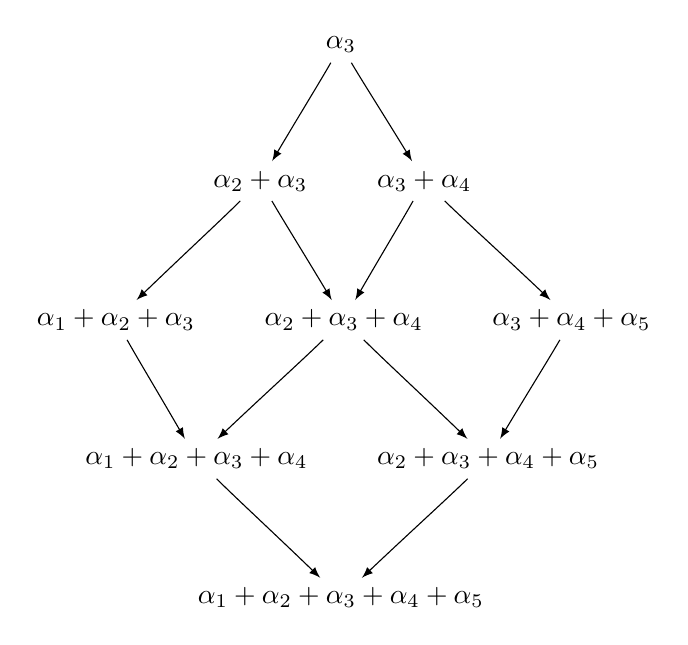
\begin{tikzpicture}[>=latex,line join=bevel,]
%%
\node (alpha3) at (113bp,206bp) [draw,draw=none] {$\alpha_{3}$};
  \node (alpha2+alpha3+alpha4+alpha5) at (166bp,57bp) [draw,draw=none] {$\alpha_{2} + \alpha_{3} + \alpha_{4} + \alpha_{5}$};
  \node (alpha2+alpha3+alpha4) at (114bp,107bp) [draw,draw=none] {$\alpha_{2} + \alpha_{3} + \alpha_{4}$};
  \node (alpha1+alpha2+alpha3+alpha4) at (61bp,57bp) [draw,draw=none] {$\alpha_{1} + \alpha_{2} + \alpha_{3} + \alpha_{4}$};
  \node (alpha2+alpha3) at (84bp,157bp) [draw,draw=none] {$\alpha_{2} + \alpha_{3}$};
  \node (alpha1+alpha2+alpha3) at (32bp,107bp) [draw,draw=none] {$\alpha_{1} + \alpha_{2} + \alpha_{3}$};
  \node (alpha1+alpha2+alpha3+alpha4+alpha5) at (113bp,7bp) [draw,draw=none] {$\alpha_{1} + \alpha_{2} + \alpha_{3} + \alpha_{4} + \alpha_{5}$};
  \node (alpha3+alpha4) at (143bp,157bp) [draw,draw=none] {$\alpha_{3} + \alpha_{4}$};
  \node (alpha3+alpha4+alpha5) at (196bp,107bp) [draw,draw=none] {$\alpha_{3} + \alpha_{4} + \alpha_{5}$};
  \draw [black,->] (alpha2+alpha3+alpha4+alpha5) ..controls (151.01bp,42.426bp) and (137.5bp,30.186bp)  .. (alpha1+alpha2+alpha3+alpha4+alpha5);
  \draw [black,->] (alpha3) ..controls (120.34bp,193.5bp) and (127.69bp,181.99bp)  .. (alpha3+alpha4);
  \draw [black,->] (alpha3+alpha4) ..controls (157.99bp,142.43bp) and (171.5bp,130.19bp)  .. (alpha3+alpha4+alpha5);
  \draw [black,->] (alpha1+alpha2+alpha3) ..controls (39.895bp,92.932bp) and (46.585bp,81.859bp)  .. (alpha1+alpha2+alpha3+alpha4);
  \draw [black,->] (alpha2+alpha3) ..controls (69.373bp,142.5bp) and (56.296bp,130.43bp)  .. (alpha1+alpha2+alpha3);
  \draw [black,->] (alpha2+alpha3) ..controls (92.168bp,142.93bp) and (99.088bp,131.86bp)  .. (alpha2+alpha3+alpha4);
  \draw [black,->] (alpha2+alpha3+alpha4) ..controls (99.012bp,92.426bp) and (85.497bp,80.186bp)  .. (alpha1+alpha2+alpha3+alpha4);
  \draw [black,->] (alpha3+alpha4+alpha5) ..controls (187.83bp,92.932bp) and (180.91bp,81.859bp)  .. (alpha2+alpha3+alpha4+alpha5);
  \draw [black,->] (alpha3) ..controls (105.91bp,193.5bp) and (98.803bp,181.99bp)  .. (alpha2+alpha3);
  \draw [black,->] (alpha3+alpha4) ..controls (135.1bp,142.93bp) and (128.41bp,131.86bp)  .. (alpha2+alpha3+alpha4);
  \draw [black,->] (alpha2+alpha3+alpha4) ..controls (128.63bp,92.498bp) and (141.7bp,80.428bp)  .. (alpha2+alpha3+alpha4+alpha5);
  \draw [black,->] (alpha1+alpha2+alpha3+alpha4) ..controls (75.627bp,42.498bp) and (88.704bp,30.428bp)  .. (alpha1+alpha2+alpha3+alpha4+alpha5);
%
\end{tikzpicture} 
	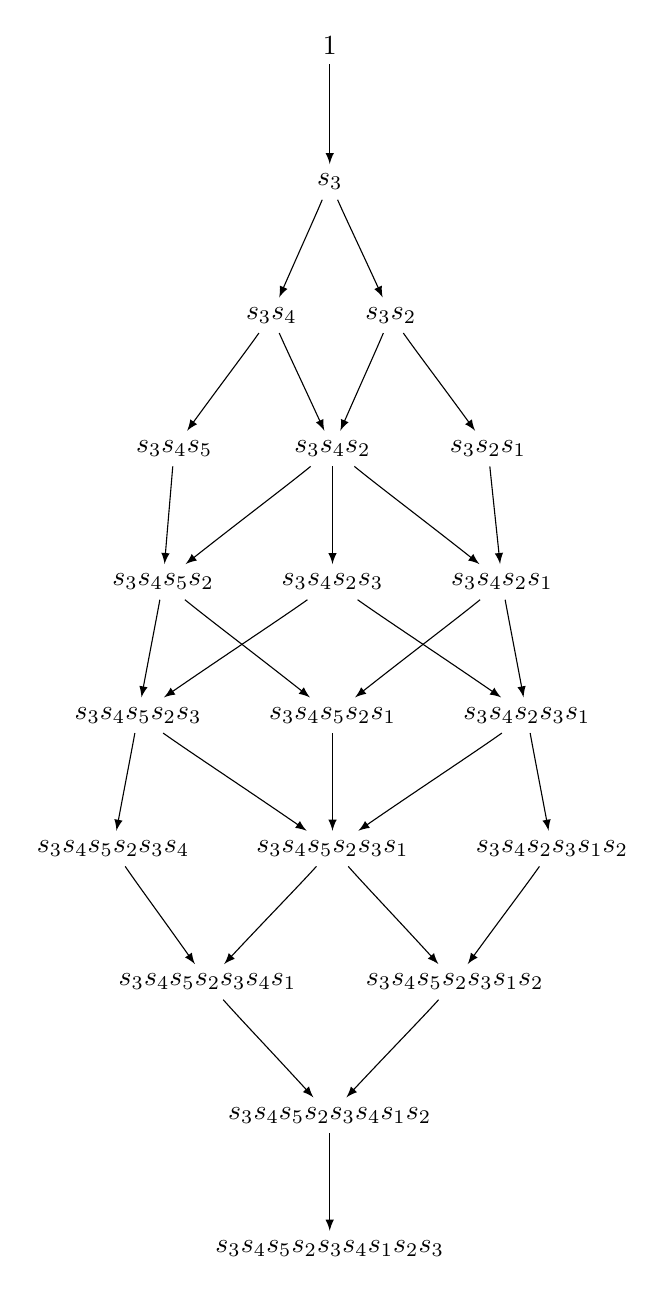
\begin{tikzpicture}[>=latex,line join=bevel,]
%%
\node (s3*s4*s5*s2*s3*s4) at (30bp,150bp) [draw,draw=none] {$s_{3}s_{4}s_{5}s_{2}s_{3}s_{4}$};
  \node (s3*s4*s5*s2*s3*s4*s1*s2) at (108bp,54bp) [draw,draw=none] {$s_{3}s_{4}s_{5}s_{2}s_{3}s_{4}s_{1}s_{2}$};
  \node (s3*s4*s5*s2*s3*s1) at (109bp,150bp) [draw,draw=none] {$s_{3}s_{4}s_{5}s_{2}s_{3}s_{1}$};
  \node (s3*s4*s5) at (52bp,294bp) [draw,draw=none] {$s_{3}s_{4}s_{5}$};
  \node (s3) at (108bp,390bp) [draw,draw=none] {$s_{3}$};
  \node (s3*s4*s5*s2*s3*s4*s1*s2*s3) at (108bp,6bp) [draw,draw=none] {$s_{3}s_{4}s_{5}s_{2}s_{3}s_{4}s_{1}s_{2}s_{3}$};
  \node (s3*s4*s2) at (109bp,294bp) [draw,draw=none] {$s_{3}s_{4}s_{2}$};
  \node (s3*s4*s5*s2*s3) at (39bp,198bp) [draw,draw=none] {$s_{3}s_{4}s_{5}s_{2}s_{3}$};
  \node (s3*s4*s5*s2) at (48bp,246bp) [draw,draw=none] {$s_{3}s_{4}s_{5}s_{2}$};
  \node (s3*s4*s5*s2*s1) at (109bp,198bp) [draw,draw=none] {$s_{3}s_{4}s_{5}s_{2}s_{1}$};
  \node (s3*s4*s5*s2*s3*s4*s1) at (64bp,102bp) [draw,draw=none] {$s_{3}s_{4}s_{5}s_{2}s_{3}s_{4}s_{1}$};
  \node (1) at (108bp,439bp) [draw,draw=none] {$1$};
  \node (s3*s4*s2*s3*s1*s2) at (188bp,150bp) [draw,draw=none] {$s_{3}s_{4}s_{2}s_{3}s_{1}s_{2}$};
  \node (s3*s4*s5*s2*s3*s1*s2) at (153bp,102bp) [draw,draw=none] {$s_{3}s_{4}s_{5}s_{2}s_{3}s_{1}s_{2}$};
  \node (s3*s2) at (130bp,342bp) [draw,draw=none] {$s_{3}s_{2}$};
  \node (s3*s2*s1) at (165bp,294bp) [draw,draw=none] {$s_{3}s_{2}s_{1}$};
  \node (s3*s4) at (87bp,342bp) [draw,draw=none] {$s_{3}s_{4}$};
  \node (s3*s4*s2*s3) at (109bp,246bp) [draw,draw=none] {$s_{3}s_{4}s_{2}s_{3}$};
  \node (s3*s4*s2*s3*s1) at (179bp,198bp) [draw,draw=none] {$s_{3}s_{4}s_{2}s_{3}s_{1}$};
  \node (s3*s4*s2*s1) at (170bp,246bp) [draw,draw=none] {$s_{3}s_{4}s_{2}s_{1}$};
  \draw [black,->] (s3*s2) ..controls (139.08bp,329.07bp) and (147.96bp,317.39bp)  .. (s3*s2*s1);
  \draw [black,->] (s3*s4*s5*s2) ..controls (64.466bp,232.58bp) and (81.602bp,219.66bp)  .. (s3*s4*s5*s2*s1);
  \draw [black,->] (s3*s4) ..controls (92.574bp,329.35bp) and (97.83bp,318.35bp)  .. (s3*s4*s2);
  \draw [black,->] (s3*s4*s5*s2*s3*s1) ..controls (97.124bp,136.86bp) and (85.185bp,124.66bp)  .. (s3*s4*s5*s2*s3*s4*s1);
  \draw [black,->] (s3*s4*s5*s2*s3) ..controls (57.738bp,184.69bp) and (78.077bp,171.32bp)  .. (s3*s4*s5*s2*s3*s1);
  \draw [black,->] (s3*s4*s2*s1) ..controls (172.24bp,233.55bp) and (174.29bp,223.07bp)  .. (s3*s4*s2*s3*s1);
  \draw [black,->] (s3*s4*s2*s3*s1) ..controls (181.24bp,185.55bp) and (183.29bp,175.07bp)  .. (s3*s4*s2*s3*s1*s2);
  \draw [black,->] (s3*s4*s5*s2*s3*s1*s2) ..controls (141.12bp,88.86bp) and (129.18bp,76.656bp)  .. (s3*s4*s5*s2*s3*s4*s1*s2);
  \draw [black,->] (s3*s4*s5*s2*s1) ..controls (109bp,185.55bp) and (109bp,175.07bp)  .. (s3*s4*s5*s2*s3*s1);
  \draw [black,->] (s3*s4*s2) ..controls (92.534bp,280.58bp) and (75.398bp,267.66bp)  .. (s3*s4*s5*s2);
  \draw [black,->] (1) ..controls (108bp,425.83bp) and (108bp,415.21bp)  .. (s3);
  \draw [black,->] (s3*s4*s2*s3*s1*s2) ..controls (178.92bp,137.07bp) and (170.04bp,125.39bp)  .. (s3*s4*s5*s2*s3*s1*s2);
  \draw [black,->] (s3*s2) ..controls (124.68bp,329.35bp) and (119.66bp,318.35bp)  .. (s3*s4*s2);
  \draw [black,->] (s3*s4*s5*s2*s3*s4*s1*s2) ..controls (108bp,41.554bp) and (108bp,31.067bp)  .. (s3*s4*s5*s2*s3*s4*s1*s2*s3);
  \draw [black,->] (s3) ..controls (113.57bp,377.35bp) and (118.83bp,366.35bp)  .. (s3*s2);
  \draw [black,->] (s3*s4*s2) ..controls (125.47bp,280.58bp) and (142.6bp,267.66bp)  .. (s3*s4*s2*s1);
  \draw [black,->] (s3*s4*s5*s2) ..controls (45.76bp,233.55bp) and (43.709bp,223.07bp)  .. (s3*s4*s5*s2*s3);
  \draw [black,->] (s3*s4*s2*s3) ..controls (127.74bp,232.69bp) and (148.08bp,219.32bp)  .. (s3*s4*s2*s3*s1);
  \draw [black,->] (s3*s4*s5*s2*s3*s4*s1) ..controls (75.546bp,88.93bp) and (87.051bp,76.902bp)  .. (s3*s4*s5*s2*s3*s4*s1*s2);
  \draw [black,->] (s3*s4*s5) ..controls (51.005bp,281.55bp) and (50.093bp,271.07bp)  .. (s3*s4*s5*s2);
  \draw [black,->] (s3*s4*s5*s2*s3) ..controls (36.76bp,185.55bp) and (34.709bp,175.07bp)  .. (s3*s4*s5*s2*s3*s4);
  \draw [black,->] (s3*s4*s5*s2*s3*s4) ..controls (38.768bp,137.14bp) and (47.271bp,125.63bp)  .. (s3*s4*s5*s2*s3*s4*s1);
  \draw [black,->] (s3*s4*s2*s3) ..controls (90.262bp,232.69bp) and (69.923bp,219.32bp)  .. (s3*s4*s5*s2*s3);
  \draw [black,->] (s3*s4*s5*s2*s3*s1) ..controls (120.55bp,136.93bp) and (132.05bp,124.9bp)  .. (s3*s4*s5*s2*s3*s1*s2);
  \draw [black,->] (s3*s4*s2*s3*s1) ..controls (160.26bp,184.69bp) and (139.92bp,171.32bp)  .. (s3*s4*s5*s2*s3*s1);
  \draw [black,->] (s3) ..controls (102.68bp,377.35bp) and (97.662bp,366.35bp)  .. (s3*s4);
  \draw [black,->] (s3*s4) ..controls (77.922bp,329.07bp) and (69.036bp,317.39bp)  .. (s3*s4*s5);
  \draw [black,->] (s3*s2*s1) ..controls (166.24bp,281.55bp) and (167.38bp,271.07bp)  .. (s3*s4*s2*s1);
  \draw [black,->] (s3*s4*s2) ..controls (109bp,281.55bp) and (109bp,271.07bp)  .. (s3*s4*s2*s3);
  \draw [black,->] (s3*s4*s2*s1) ..controls (153.53bp,232.58bp) and (136.4bp,219.66bp)  .. (s3*s4*s5*s2*s1);
%
\end{tikzpicture} 
	}
  \caption{Poset of noncompact roots and the Bruhat graph for $\mathrm{SU}(3,3)$}
\end{figure} 

\begin{figure}[H]
  \centering 
  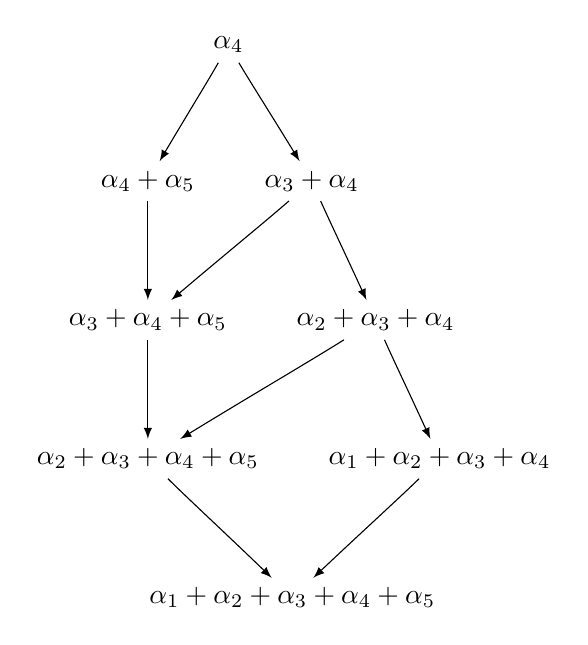
\begin{tikzpicture}[>=latex,line join=bevel,]
%%
\node (alpha2+alpha3+alpha4+alpha5) at (43bp,57bp) [draw,draw=none] {$\alpha_{2} + \alpha_{3} + \alpha_{4} + \alpha_{5}$};
  \node (alpha2+alpha3+alpha4) at (125bp,107bp) [draw,draw=none] {$\alpha_{2} + \alpha_{3} + \alpha_{4}$};
  \node (alpha4) at (72bp,206bp) [draw,draw=none] {$\alpha_{4}$};
  \node (alpha1+alpha2+alpha3+alpha4) at (148bp,57bp) [draw,draw=none] {$\alpha_{1} + \alpha_{2} + \alpha_{3} + \alpha_{4}$};
  \node (alpha4+alpha5) at (43bp,157bp) [draw,draw=none] {$\alpha_{4} + \alpha_{5}$};
  \node (alpha1+alpha2+alpha3+alpha4+alpha5) at (95bp,7bp) [draw,draw=none] {$\alpha_{1} + \alpha_{2} + \alpha_{3} + \alpha_{4} + \alpha_{5}$};
  \node (alpha3+alpha4) at (102bp,157bp) [draw,draw=none] {$\alpha_{3} + \alpha_{4}$};
  \node (alpha3+alpha4+alpha5) at (43bp,107bp) [draw,draw=none] {$\alpha_{3} + \alpha_{4} + \alpha_{5}$};
  \draw [black,->] (alpha2+alpha3+alpha4) ..controls (131.19bp,93.076bp) and (136.34bp,82.328bp)  .. (alpha1+alpha2+alpha3+alpha4);
  \draw [black,->] (alpha2+alpha3+alpha4+alpha5) ..controls (57.627bp,42.498bp) and (70.704bp,30.428bp)  .. (alpha1+alpha2+alpha3+alpha4+alpha5);
  \draw [black,->] (alpha1+alpha2+alpha3+alpha4) ..controls (133.01bp,42.426bp) and (119.5bp,30.186bp)  .. (alpha1+alpha2+alpha3+alpha4+alpha5);
  \draw [black,->] (alpha4) ..controls (64.906bp,193.5bp) and (57.803bp,181.99bp)  .. (alpha4+alpha5);
  \draw [black,->] (alpha4+alpha5) ..controls (43bp,143.29bp) and (43bp,133.02bp)  .. (alpha3+alpha4+alpha5);
  \draw [black,->] (alpha3+alpha4+alpha5) ..controls (43bp,93.293bp) and (43bp,83.024bp)  .. (alpha2+alpha3+alpha4+alpha5);
  \draw [black,->] (alpha3+alpha4) ..controls (108.19bp,143.08bp) and (113.34bp,132.33bp)  .. (alpha2+alpha3+alpha4);
  \draw [black,->] (alpha4) ..controls (79.339bp,193.5bp) and (86.686bp,181.99bp)  .. (alpha3+alpha4);
  \draw [black,->] (alpha3+alpha4) ..controls (85.226bp,142.35bp) and (69.971bp,129.94bp)  .. (alpha3+alpha4+alpha5);
  \draw [black,->] (alpha2+alpha3+alpha4) ..controls (101.43bp,92.203bp) and (78.43bp,78.739bp)  .. (alpha2+alpha3+alpha4+alpha5);
%
\end{tikzpicture} 
	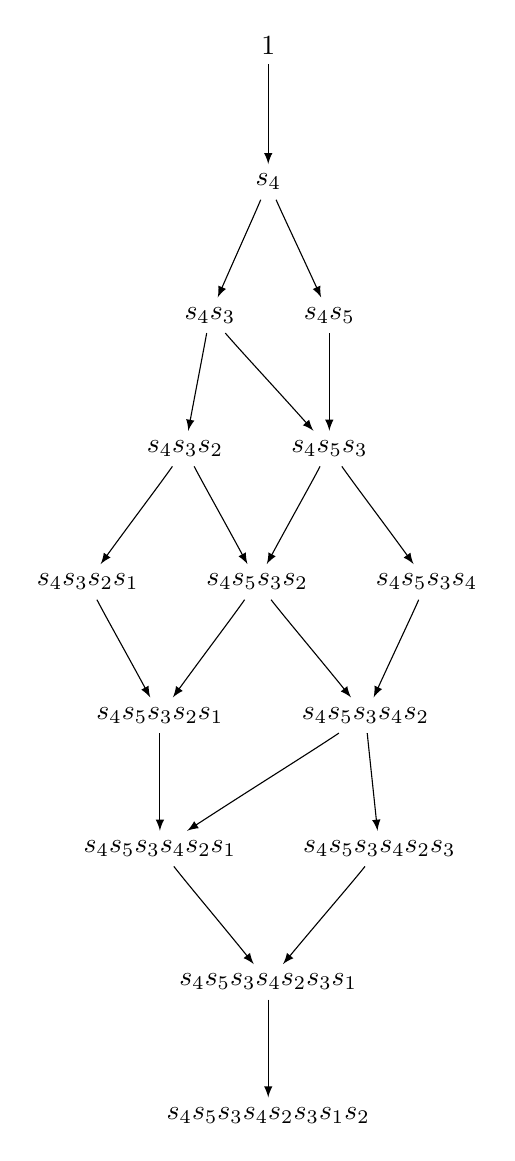
\begin{tikzpicture}[>=latex,line join=bevel,]
%%
\node (s4*s5*s3*s4*s2*s3) at (126bp,102bp) [draw,draw=none] {$s_{4}s_{5}s_{3}s_{4}s_{2}s_{3}$};
  \node (s4*s5*s3*s4) at (143bp,198bp) [draw,draw=none] {$s_{4}s_{5}s_{3}s_{4}$};
  \node (s4*s5*s3*s4*s2*s1) at (47bp,102bp) [draw,draw=none] {$s_{4}s_{5}s_{3}s_{4}s_{2}s_{1}$};
  \node (s4*s5*s3*s2) at (82bp,198bp) [draw,draw=none] {$s_{4}s_{5}s_{3}s_{2}$};
  \node (s4*s3*s2) at (56bp,246bp) [draw,draw=none] {$s_{4}s_{3}s_{2}$};
  \node (s4*s3) at (65bp,294bp) [draw,draw=none] {$s_{4}s_{3}$};
  \node (s4*s5) at (108bp,294bp) [draw,draw=none] {$s_{4}s_{5}$};
  \node (s4*s5*s3*s4*s2*s3*s1) at (86bp,54bp) [draw,draw=none] {$s_{4}s_{5}s_{3}s_{4}s_{2}s_{3}s_{1}$};
  \node (s4) at (86bp,342bp) [draw,draw=none] {$s_{4}$};
  \node (1) at (86bp,391bp) [draw,draw=none] {$1$};
  \node (s4*s5*s3*s4*s2) at (121bp,150bp) [draw,draw=none] {$s_{4}s_{5}s_{3}s_{4}s_{2}$};
  \node (s4*s5*s3*s2*s1) at (47bp,150bp) [draw,draw=none] {$s_{4}s_{5}s_{3}s_{2}s_{1}$};
  \node (s4*s5*s3*s4*s2*s3*s1*s2) at (86bp,6bp) [draw,draw=none] {$s_{4}s_{5}s_{3}s_{4}s_{2}s_{3}s_{1}s_{2}$};
  \node (s4*s5*s3) at (108bp,246bp) [draw,draw=none] {$s_{4}s_{5}s_{3}$};
  \node (s4*s3*s2*s1) at (21bp,198bp) [draw,draw=none] {$s_{4}s_{3}s_{2}s_{1}$};
  \draw [black,->] (s4*s5*s3*s2) ..controls (72.922bp,185.07bp) and (64.036bp,173.39bp)  .. (s4*s5*s3*s2*s1);
  \draw [black,->] (s4*s3) ..controls (62.76bp,281.55bp) and (60.709bp,271.07bp)  .. (s4*s3*s2);
  \draw [black,->] (s4*s5*s3) ..controls (117.08bp,233.07bp) and (125.96bp,221.39bp)  .. (s4*s5*s3*s4);
  \draw [black,->] (s4*s3*s2) ..controls (62.626bp,233.28bp) and (68.935bp,222.12bp)  .. (s4*s5*s3*s2);
  \draw [black,->] (s4*s5) ..controls (108bp,281.55bp) and (108bp,271.07bp)  .. (s4*s5*s3);
  \draw [black,->] (s4*s5*s3*s2*s1) ..controls (47bp,137.55bp) and (47bp,127.07bp)  .. (s4*s5*s3*s4*s2*s1);
  \draw [black,->] (s4*s3*s2*s1) ..controls (27.626bp,185.28bp) and (33.935bp,174.12bp)  .. (s4*s5*s3*s2*s1);
  \draw [black,->] (s4) ..controls (91.574bp,329.35bp) and (96.83bp,318.35bp)  .. (s4*s5);
  \draw [black,->] (s4*s5*s3*s4*s2*s3) ..controls (115.56bp,88.999bp) and (105.26bp,77.147bp)  .. (s4*s5*s3*s4*s2*s3*s1);
  \draw [black,->] (s4*s5*s3*s4*s2*s1) ..controls (57.175bp,88.999bp) and (67.224bp,77.147bp)  .. (s4*s5*s3*s4*s2*s3*s1);
  \draw [black,->] (s4) ..controls (80.68bp,329.35bp) and (75.662bp,318.35bp)  .. (s4*s3);
  \draw [black,->] (s4*s5*s3*s4) ..controls (137.43bp,185.35bp) and (132.17bp,174.35bp)  .. (s4*s5*s3*s4*s2);
  \draw [black,->] (s4*s5*s3*s4*s2) ..controls (101.08bp,136.62bp) and (79.28bp,123.07bp)  .. (s4*s5*s3*s4*s2*s1);
  \draw [black,->] (s4*s5*s3) ..controls (101.37bp,233.28bp) and (95.065bp,222.12bp)  .. (s4*s5*s3*s2);
  \draw [black,->] (s4*s5*s3*s4*s2) ..controls (122.24bp,137.55bp) and (123.38bp,127.07bp)  .. (s4*s5*s3*s4*s2*s3);
  \draw [black,->] (s4*s3) ..controls (76.283bp,280.93bp) and (87.527bp,268.9bp)  .. (s4*s5*s3);
  \draw [black,->] (1) ..controls (86bp,377.83bp) and (86bp,367.21bp)  .. (s4);
  \draw [black,->] (s4*s5*s3*s2) ..controls (92.175bp,185bp) and (102.22bp,173.15bp)  .. (s4*s5*s3*s4*s2);
  \draw [black,->] (s4*s3*s2) ..controls (46.922bp,233.07bp) and (38.036bp,221.39bp)  .. (s4*s3*s2*s1);
  \draw [black,->] (s4*s5*s3*s4*s2*s3*s1) ..controls (86bp,41.554bp) and (86bp,31.067bp)  .. (s4*s5*s3*s4*s2*s3*s1*s2);
%
\end{tikzpicture} 
  \caption{Poset of noncompact roots and the Bruhat graph for $\mathrm{SU}(4,2)$}
\end{figure} 

\begin{figure}[H]
  \centering 
  \begin{tikzpicture}[>=latex,line join=bevel,]
%%
\node (alpha1+alpha2+alpha3+alpha4+alpha5) at (55bp,7bp) [draw,draw=none] {$\alpha_{1} + \alpha_{2} + \alpha_{3} + \alpha_{4} + \alpha_{5}$};
  \node (alpha2+alpha3+alpha4+alpha5) at (55bp,57bp) [draw,draw=none] {$\alpha_{2} + \alpha_{3} + \alpha_{4} + \alpha_{5}$};
  \node (alpha5) at (55bp,206bp) [draw,draw=none] {$\alpha_{5}$};
  \node (alpha3+alpha4+alpha5) at (55bp,107bp) [draw,draw=none] {$\alpha_{3} + \alpha_{4} + \alpha_{5}$};
  \node (alpha4+alpha5) at (55bp,157bp) [draw,draw=none] {$\alpha_{4} + \alpha_{5}$};
  \draw [black,->] (alpha4+alpha5) ..controls (55bp,143.29bp) and (55bp,133.02bp)  .. (alpha3+alpha4+alpha5);
  \draw [black,->] (alpha3+alpha4+alpha5) ..controls (55bp,93.293bp) and (55bp,83.024bp)  .. (alpha2+alpha3+alpha4+alpha5);
  \draw [black,->] (alpha5) ..controls (55bp,193.84bp) and (55bp,183.19bp)  .. (alpha4+alpha5);
  \draw [black,->] (alpha2+alpha3+alpha4+alpha5) ..controls (55bp,43.293bp) and (55bp,33.024bp)  .. (alpha1+alpha2+alpha3+alpha4+alpha5);
%
\end{tikzpicture}
	\begin{tikzpicture}[>=latex,line join=bevel,]
%%
\node (s5*s4*s3*s2*s1) at (26bp,6bp) [draw,draw=none] {$s_{5}s_{4}s_{3}s_{2}s_{1}$};
  \node (s5) at (26bp,198bp) [draw,draw=none] {$s_{5}$};
  \node (1) at (26bp,247bp) [draw,draw=none] {$1$};
  \node (s5*s4*s3*s2) at (26bp,54bp) [draw,draw=none] {$s_{5}s_{4}s_{3}s_{2}$};
  \node (s5*s4*s3) at (26bp,102bp) [draw,draw=none] {$s_{5}s_{4}s_{3}$};
  \node (s5*s4) at (26bp,150bp) [draw,draw=none] {$s_{5}s_{4}$};
  \draw [black,->] (s5*s4*s3*s2) ..controls (26bp,41.554bp) and (26bp,31.067bp)  .. (s5*s4*s3*s2*s1);
  \draw [black,->] (1) ..controls (26bp,233.83bp) and (26bp,223.21bp)  .. (s5);
  \draw [black,->] (s5) ..controls (26bp,185.55bp) and (26bp,175.07bp)  .. (s5*s4);
  \draw [black,->] (s5*s4*s3) ..controls (26bp,89.554bp) and (26bp,79.067bp)  .. (s5*s4*s3*s2);
  \draw [black,->] (s5*s4) ..controls (26bp,137.55bp) and (26bp,127.07bp)  .. (s5*s4*s3);
%
\end{tikzpicture}
  \caption{Poset of noncompact roots and the Bruhat graph for $\mathrm{SU}(5,1)$}
\end{figure} 

\begin{figure}[H]
  \centering 
  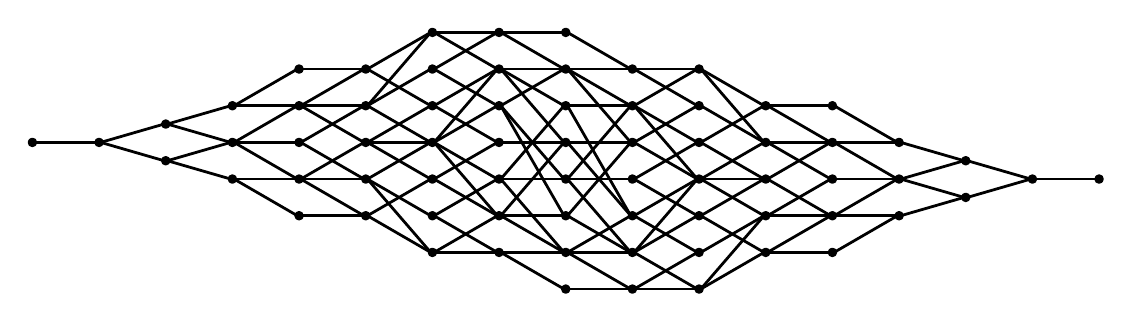
\begin{tikzpicture}[=latex,line join=bevel,scale=0.6]
  \pgfsetlinewidth{1bp}
%%
\pgfsetcolor{black}
  % Edge: s_4*s_5*s_6*s_7*s_3*s_4*s_5*s_2 - s_4*s_5*s_6*s_7*s_3*s_4*s_5*s_2*s_3
  \draw [-] (323.94bp,132.46bp) .. controls (327.67bp,130.3bp) and (341.69bp,122.18bp)  .. (360.22bp,111.45bp);
  % Edge: s_4*s_5*s_6*s_3*s_4*s_2*s_3 - s_4*s_5*s_6*s_3*s_4*s_5*s_2*s_3
  \draw [-] (283.94bp,67bp) .. controls (287.42bp,67bp) and (299.87bp,67bp)  .. (319.65bp,67bp);
  % Edge: s_4*s_5*s_3 - s_4*s_5*s_3*s_2
  \draw [-] (123.94bp,88.456bp) .. controls (127.67bp,86.297bp) and (141.69bp,78.178bp)  .. (160.22bp,67.449bp);
  % Edge: s_4*s_5*s_6*s_3*s_4*s_5*s_2*s_3*s_4 - s_4*s_5*s_6*s_7*s_3*s_4*s_5*s_2*s_3*s_4
  \draw [-] (363.94bp,67.544bp) .. controls (367.67bp,69.703bp) and (381.69bp,77.822bp)  .. (400.22bp,88.551bp);
  % Edge: s_4*s_5*s_6*s_7*s_3*s_4*s_5*s_6*s_2*s_3*s_4*s_1 - s_4*s_5*s_6*s_7*s_3*s_4*s_5*s_6*s_2*s_3*s_4*s_1*s_2
  \draw [-] (483.94bp,88.456bp) .. controls (487.67bp,86.297bp) and (501.69bp,78.178bp)  .. (520.22bp,67.449bp);
  % Edge: s_4 - s_4*s_3
  \draw [-] (43.939bp,88.728bp) .. controls (47.499bp,87.698bp) and (60.446bp,83.95bp)  .. (79.648bp,78.391bp);
  % Edge: s_4*s_5*s_6*s_7*s_3*s_2*s_1 - s_4*s_5*s_6*s_7*s_3*s_4*s_2*s_1
  \draw [-] (283.94bp,89bp) .. controls (287.42bp,89bp) and (299.87bp,89bp)  .. (319.65bp,89bp);
  % Edge: s_4*s_5*s_6*s_7*s_3*s_4*s_5*s_6*s_2*s_3*s_4*s_1*s_2 - s_4*s_5*s_6*s_7*s_3*s_4*s_5*s_6*s_2*s_3*s_4*s_1*s_2*s_3
  \draw [-] (523.94bp,66.728bp) .. controls (527.5bp,65.698bp) and (540.45bp,61.95bp)  .. (559.65bp,56.391bp);
  % Edge: s_4*s_5*s_6*s_3*s_4*s_5*s_2*s_1 - s_4*s_5*s_6*s_7*s_3*s_4*s_5*s_2*s_1
  \draw [-] (323.66bp,45.764bp) .. controls (327.16bp,49.818bp) and (343.78bp,69.061bp)  .. (360.2bp,88.071bp);
  % Edge: s_4*s_5*s_6*s_7*s_3*s_4*s_5*s_6*s_2*s_3*s_4*s_1*s_2 - s_4*s_5*s_6*s_7*s_3*s_4*s_5*s_6*s_2*s_3*s_4*s_5*s_1*s_2
  \draw [-] (523.94bp,67.272bp) .. controls (527.5bp,68.302bp) and (540.45bp,72.05bp)  .. (559.65bp,77.609bp);
  % Edge: s_4*s_5*s_3*s_2*s_1 - s_4*s_5*s_3*s_4*s_2*s_1
  \draw [-] (203.94bp,44.456bp) .. controls (207.67bp,42.297bp) and (221.69bp,34.178bp)  .. (240.22bp,23.449bp);
  % Edge: s_4*s_5*s_6*s_7*s_3*s_4*s_2*s_3 - s_4*s_5*s_6*s_7*s_3*s_4*s_5*s_2*s_3
  \draw [-] (323.94bp,111bp) .. controls (327.42bp,111bp) and (339.87bp,111bp)  .. (359.65bp,111bp);
  % Edge: s_4*s_5*s_6*s_7*s_3*s_4*s_5*s_2*s_3*s_4*s_1*s_2 - s_4*s_5*s_6*s_7*s_3*s_4*s_5*s_2*s_3*s_4*s_1*s_2*s_3
  \draw [-] (483.94bp,45bp) .. controls (487.42bp,45bp) and (499.87bp,45bp)  .. (519.65bp,45bp);
  % Edge: s_4*s_5*s_6*s_3*s_4*s_5 - s_4*s_5*s_6*s_3*s_4*s_5*s_2
  \draw [-] (243.94bp,132.46bp) .. controls (247.67bp,130.3bp) and (261.69bp,122.18bp)  .. (280.22bp,111.45bp);
  % Edge: s_4*s_5*s_6*s_7*s_3*s_4*s_5*s_6*s_2*s_3*s_1 - s_4*s_5*s_6*s_7*s_3*s_4*s_5*s_6*s_2*s_3*s_1*s_2
  \draw [-] (443.94bp,88.456bp) .. controls (447.67bp,86.297bp) and (461.69bp,78.178bp)  .. (480.22bp,67.449bp);
  % Edge: s_4*s_5*s_3*s_2*s_1 - s_4*s_5*s_6*s_3*s_2*s_1
  \draw [-] (203.94bp,45.544bp) .. controls (207.67bp,47.703bp) and (221.69bp,55.822bp)  .. (240.22bp,66.551bp);
  % Edge: s_4*s_5*s_6*s_3*s_2 - s_4*s_5*s_6*s_3*s_2*s_1
  \draw [-] (203.94bp,88.456bp) .. controls (207.67bp,86.297bp) and (221.69bp,78.178bp)  .. (240.22bp,67.449bp);
  % Edge: s_4*s_5*s_6*s_7*s_3 - s_4*s_5*s_6*s_7*s_3*s_2
  \draw [-] (203.94bp,132.46bp) .. controls (207.67bp,130.3bp) and (221.69bp,122.18bp)  .. (240.22bp,111.45bp);
  % Edge: s_4*s_5*s_6*s_3 - s_4*s_5*s_6*s_7*s_3
  \draw [-] (163.94bp,111.54bp) .. controls (167.67bp,113.7bp) and (181.69bp,121.82bp)  .. (200.22bp,132.55bp);
  % Edge: s_4*s_5*s_6*s_3*s_4 - s_4*s_5*s_6*s_7*s_3*s_4
  \draw [-] (203.66bp,111.76bp) .. controls (207.16bp,115.82bp) and (223.78bp,135.06bp)  .. (240.2bp,154.07bp);
  % Edge: s_4*s_5*s_6*s_7*s_3*s_4*s_5*s_6*s_2*s_3*s_4*s_5*s_1 - s_4*s_5*s_6*s_7*s_3*s_4*s_5*s_6*s_2*s_3*s_4*s_5*s_1*s_2
  \draw [-] (523.94bp,88.728bp) .. controls (527.5bp,87.698bp) and (540.45bp,83.95bp)  .. (559.65bp,78.391bp);
  % Edge: s_4*s_5*s_6*s_7*s_3*s_4*s_2*s_3*s_1 - s_4*s_5*s_6*s_7*s_3*s_4*s_5*s_2*s_3*s_1
  \draw [-] (363.94bp,45.544bp) .. controls (367.67bp,47.703bp) and (381.69bp,55.822bp)  .. (400.22bp,66.551bp);
  % Edge: s_4*s_5*s_6*s_3*s_2*s_1 - s_4*s_5*s_6*s_7*s_3*s_2*s_1
  \draw [-] (243.94bp,67.544bp) .. controls (247.67bp,69.703bp) and (261.69bp,77.822bp)  .. (280.22bp,88.551bp);
  % Edge: s_4*s_5*s_6*s_7*s_3*s_4*s_5*s_2*s_1 - s_4*s_5*s_6*s_7*s_3*s_4*s_5*s_6*s_2*s_1
  \draw [-] (363.94bp,89.544bp) .. controls (367.67bp,91.703bp) and (381.69bp,99.822bp)  .. (400.22bp,110.55bp);
  % Edge: s_4*s_5*s_6*s_7*s_3*s_4*s_5*s_2*s_3*s_1 - s_4*s_5*s_6*s_7*s_3*s_4*s_5*s_2*s_3*s_4*s_1
  \draw [-] (403.94bp,67bp) .. controls (407.42bp,67bp) and (419.87bp,67bp)  .. (439.65bp,67bp);
  % Edge: s_4*s_5*s_6*s_3*s_4*s_2 - s_4*s_5*s_6*s_7*s_3*s_4*s_2
  \draw [-] (243.66bp,89.764bp) .. controls (247.16bp,93.818bp) and (263.78bp,113.06bp)  .. (280.2bp,132.07bp);
  % Edge: s_4*s_5*s_6*s_7*s_3*s_4*s_5*s_6*s_2*s_3*s_4*s_5 - s_4*s_5*s_6*s_7*s_3*s_4*s_5*s_6*s_2*s_3*s_4*s_5*s_1
  \draw [-] (483.94bp,110.46bp) .. controls (487.67bp,108.3bp) and (501.69bp,100.18bp)  .. (520.22bp,89.449bp);
  % Edge: s_4*s_5*s_6*s_7*s_3*s_4*s_5*s_2*s_3*s_4*s_1 - s_4*s_5*s_6*s_7*s_3*s_4*s_5*s_2*s_3*s_4*s_1*s_2
  \draw [-] (443.94bp,66.456bp) .. controls (447.67bp,64.297bp) and (461.69bp,56.178bp)  .. (480.22bp,45.449bp);
  % Edge: s_4*s_5*s_6*s_3*s_4*s_5*s_2*s_3*s_1*s_2 - s_4*s_5*s_6*s_7*s_3*s_4*s_5*s_2*s_3*s_1*s_2
  \draw [-] (403.66bp,1.7637bp) .. controls (407.16bp,5.8177bp) and (423.78bp,25.061bp)  .. (440.2bp,44.071bp);
  % Edge: s_4*s_5*s_3*s_4*s_2*s_3 - s_4*s_5*s_3*s_4*s_2*s_3*s_1
  \draw [-] (243.94bp,44.456bp) .. controls (247.67bp,42.297bp) and (261.69bp,34.178bp)  .. (280.22bp,23.449bp);
  % Edge: s_4*s_5*s_6*s_3*s_4*s_5*s_2*s_3*s_4*s_1*s_2 - s_4*s_5*s_6*s_7*s_3*s_4*s_5*s_2*s_3*s_4*s_1*s_2
  \draw [-] (443.94bp,23.544bp) .. controls (447.67bp,25.703bp) and (461.69bp,33.822bp)  .. (480.22bp,44.551bp);
  % Edge: s_4*s_5*s_6*s_7*s_3*s_4*s_5*s_6*s_2 - s_4*s_5*s_6*s_7*s_3*s_4*s_5*s_6*s_2*s_3
  \draw [-] (363.94bp,133bp) .. controls (367.42bp,133bp) and (379.87bp,133bp)  .. (399.65bp,133bp);
  % Edge: s_4*s_5*s_3*s_4*s_2 - s_4*s_5*s_3*s_4*s_2*s_3
  \draw [-] (203.94bp,66.456bp) .. controls (207.67bp,64.297bp) and (221.69bp,56.178bp)  .. (240.22bp,45.449bp);
  % Edge: s_4*s_5*s_6*s_7*s_3*s_4*s_2*s_3*s_1*s_2 - s_4*s_5*s_6*s_7*s_3*s_4*s_5*s_2*s_3*s_1*s_2
  \draw [-] (403.94bp,23.544bp) .. controls (407.67bp,25.703bp) and (421.69bp,33.822bp)  .. (440.22bp,44.551bp);
  % Edge: s_4*s_5*s_3*s_4*s_2*s_1 - s_4*s_5*s_3*s_4*s_2*s_3*s_1
  \draw [-] (243.94bp,23bp) .. controls (247.42bp,23bp) and (259.87bp,23bp)  .. (279.65bp,23bp);
  % Edge: s_4*s_5*s_6*s_3*s_4*s_2 - s_4*s_5*s_6*s_3*s_4*s_2*s_1
  \draw [-] (243.66bp,88.236bp) .. controls (247.16bp,84.182bp) and (263.78bp,64.939bp)  .. (280.2bp,45.929bp);
  % Edge: s_4*s_5*s_6*s_3*s_4*s_5*s_2*s_3*s_4*s_1 - s_4*s_5*s_6*s_3*s_4*s_5*s_2*s_3*s_4*s_1*s_2
  \draw [-] (403.94bp,44.456bp) .. controls (407.67bp,42.297bp) and (421.69bp,34.178bp)  .. (440.22bp,23.449bp);
  % Edge: s_4*s_5*s_6*s_7*s_3 - s_4*s_5*s_6*s_7*s_3*s_4
  \draw [-] (203.94bp,133.54bp) .. controls (207.67bp,135.7bp) and (221.69bp,143.82bp)  .. (240.22bp,154.55bp);
  % Edge: s_4*s_5*s_6*s_7*s_3*s_4*s_5*s_6*s_2*s_3 - s_4*s_5*s_6*s_7*s_3*s_4*s_5*s_6*s_2*s_3*s_1
  \draw [-] (403.66bp,132.24bp) .. controls (407.16bp,128.18bp) and (423.78bp,108.94bp)  .. (440.2bp,89.929bp);
  % Edge: s_4*s_5*s_6*s_3*s_4*s_2*s_3*s_1 - s_4*s_5*s_6*s_7*s_3*s_4*s_2*s_3*s_1
  \draw [-] (323.94bp,23.544bp) .. controls (327.67bp,25.703bp) and (341.69bp,33.822bp)  .. (360.22bp,44.551bp);
  % Edge: s_4*s_5*s_6*s_3 - s_4*s_5*s_6*s_3*s_4
  \draw [-] (163.94bp,111bp) .. controls (167.42bp,111bp) and (179.87bp,111bp)  .. (199.65bp,111bp);
  % Edge: s_4*s_5*s_6*s_7*s_3*s_4*s_5*s_2*s_3*s_4*s_1*s_2*s_3 - s_4*s_5*s_6*s_7*s_3*s_4*s_5*s_6*s_2*s_3*s_4*s_1*s_2*s_3
  \draw [-] (523.94bp,45.272bp) .. controls (527.5bp,46.302bp) and (540.45bp,50.05bp)  .. (559.65bp,55.609bp);
  % Edge: s_4*s_5*s_6*s_7*s_3*s_4*s_2*s_3 - s_4*s_5*s_6*s_7*s_3*s_4*s_2*s_3*s_1
  \draw [-] (323.66bp,109.85bp) .. controls (327.37bp,103.42bp) and (345.78bp,71.438bp)  .. (360.44bp,45.978bp);
  % Edge: s_4*s_5*s_6*s_3*s_4 - s_4*s_5*s_6*s_3*s_4*s_2
  \draw [-] (203.94bp,110.46bp) .. controls (207.67bp,108.3bp) and (221.69bp,100.18bp)  .. (240.22bp,89.449bp);
  % Edge: s_4*s_5*s_6*s_3*s_4*s_2*s_3*s_1*s_2 - s_4*s_5*s_6*s_7*s_3*s_4*s_2*s_3*s_1*s_2
  \draw [-] (363.94bp,1.5438bp) .. controls (367.67bp,3.7026bp) and (381.69bp,11.822bp)  .. (400.22bp,22.551bp);
  % Edge: s_4*s_5*s_6*s_7*s_3*s_4 - s_4*s_5*s_6*s_7*s_3*s_4*s_5
  \draw [-] (243.94bp,155bp) .. controls (247.42bp,155bp) and (259.87bp,155bp)  .. (279.65bp,155bp);
  % Edge: s_4*s_5*s_6*s_3*s_4*s_5*s_2*s_3*s_4*s_1*s_2*s_3 - s_4*s_5*s_6*s_7*s_3*s_4*s_5*s_2*s_3*s_4*s_1*s_2*s_3
  \draw [-] (483.94bp,23.544bp) .. controls (487.67bp,25.703bp) and (501.69bp,33.822bp)  .. (520.22bp,44.551bp);
  % Edge: s_4*s_3*s_2*s_1 - s_4*s_5*s_3*s_2*s_1
  \draw [-] (163.94bp,45bp) .. controls (167.42bp,45bp) and (179.87bp,45bp)  .. (199.65bp,45bp);
  % Edge: s_4*s_5*s_6*s_3*s_4*s_5*s_2*s_3*s_4*s_1 - s_4*s_5*s_6*s_7*s_3*s_4*s_5*s_2*s_3*s_4*s_1
  \draw [-] (403.94bp,45.544bp) .. controls (407.67bp,47.703bp) and (421.69bp,55.822bp)  .. (440.22bp,66.551bp);
  % Edge: s_4*s_5*s_6*s_7*s_3*s_4*s_5*s_6*s_2*s_3*s_4 - s_4*s_5*s_6*s_7*s_3*s_4*s_5*s_6*s_2*s_3*s_4*s_5
  \draw [-] (443.94bp,111bp) .. controls (447.42bp,111bp) and (459.87bp,111bp)  .. (479.65bp,111bp);
  % Edge: s_4*s_5*s_6*s_3*s_4*s_5*s_2*s_1 - s_4*s_5*s_6*s_3*s_4*s_5*s_2*s_3*s_1
  \draw [-] (323.94bp,44.456bp) .. controls (327.67bp,42.297bp) and (341.69bp,34.178bp)  .. (360.22bp,23.449bp);
  % Edge: s_4*s_5*s_6*s_7*s_3*s_4*s_5*s_2*s_3 - s_4*s_5*s_6*s_7*s_3*s_4*s_5*s_2*s_3*s_4
  \draw [-] (363.94bp,110.46bp) .. controls (367.67bp,108.3bp) and (381.69bp,100.18bp)  .. (400.22bp,89.449bp);
  % Edge: s_4*s_5*s_6*s_7*s_3*s_4*s_2*s_1 - s_4*s_5*s_6*s_7*s_3*s_4*s_5*s_2*s_1
  \draw [-] (323.94bp,89bp) .. controls (327.42bp,89bp) and (339.87bp,89bp)  .. (359.65bp,89bp);
  % Edge: s_4*s_5*s_6*s_3*s_4*s_5*s_2*s_3 - s_4*s_5*s_6*s_3*s_4*s_5*s_2*s_3*s_4
  \draw [-] (323.94bp,67bp) .. controls (327.42bp,67bp) and (339.87bp,67bp)  .. (359.65bp,67bp);
  % Edge: s_4*s_5*s_6*s_3*s_4*s_5*s_2 - s_4*s_5*s_6*s_7*s_3*s_4*s_5*s_2
  \draw [-] (283.94bp,111.54bp) .. controls (287.67bp,113.7bp) and (301.69bp,121.82bp)  .. (320.22bp,132.55bp);
  % Edge: s_4*s_5*s_6*s_7*s_3*s_4*s_5*s_2*s_3*s_4 - s_4*s_5*s_6*s_7*s_3*s_4*s_5*s_6*s_2*s_3*s_4
  \draw [-] (403.94bp,89.544bp) .. controls (407.67bp,91.703bp) and (421.69bp,99.822bp)  .. (440.22bp,110.55bp);
  % Edge: s_4*s_5*s_6*s_3*s_4*s_5*s_2 - s_4*s_5*s_6*s_3*s_4*s_5*s_2*s_1
  \draw [-] (283.66bp,109.85bp) .. controls (287.37bp,103.42bp) and (305.78bp,71.438bp)  .. (320.44bp,45.978bp);
  % Edge: s_4*s_5*s_3 - s_4*s_5*s_6*s_3
  \draw [-] (123.94bp,89.544bp) .. controls (127.67bp,91.703bp) and (141.69bp,99.822bp)  .. (160.22bp,110.55bp);
  % Edge: s_4*s_5*s_6*s_7*s_3*s_4*s_5*s_6*s_2*s_3*s_4*s_5*s_1*s_2*s_3 - s_4*s_5*s_6*s_7*s_3*s_4*s_5*s_6*s_2*s_3*s_4*s_5*s_1*s_2*s_3*s_4
  \draw [-] (603.94bp,67bp) .. controls (607.42bp,67bp) and (619.87bp,67bp)  .. (639.65bp,67bp);
  % Edge: s_4*s_5*s_6*s_3*s_4*s_2*s_1 - s_4*s_5*s_6*s_3*s_4*s_2*s_3*s_1
  \draw [-] (283.94bp,44.456bp) .. controls (287.67bp,42.297bp) and (301.69bp,34.178bp)  .. (320.22bp,23.449bp);
  % Edge: s_4*s_5*s_3 - s_4*s_5*s_3*s_4
  \draw [-] (123.94bp,89bp) .. controls (127.42bp,89bp) and (139.87bp,89bp)  .. (159.65bp,89bp);
  % Edge: s_4*s_5*s_6 - s_4*s_5*s_6*s_3
  \draw [-] (123.94bp,111bp) .. controls (127.42bp,111bp) and (139.87bp,111bp)  .. (159.65bp,111bp);
  % Edge: s_4*s_5*s_6*s_7*s_3*s_4*s_5*s_2*s_3*s_1 - s_4*s_5*s_6*s_7*s_3*s_4*s_5*s_6*s_2*s_3*s_1
  \draw [-] (403.94bp,67.544bp) .. controls (407.67bp,69.703bp) and (421.69bp,77.822bp)  .. (440.22bp,88.551bp);
  % Edge: s_4*s_5*s_3*s_4*s_2*s_3 - s_4*s_5*s_6*s_3*s_4*s_2*s_3
  \draw [-] (243.94bp,45.544bp) .. controls (247.67bp,47.703bp) and (261.69bp,55.822bp)  .. (280.22bp,66.551bp);
  % Edge: s_4*s_5 - s_4*s_5*s_3
  \draw [-] (83.939bp,99.728bp) .. controls (87.499bp,98.698bp) and (100.45bp,94.95bp)  .. (119.65bp,89.391bp);
  % Edge: s_4*s_5*s_6*s_3*s_4*s_5*s_2*s_3 - s_4*s_5*s_6*s_3*s_4*s_5*s_2*s_3*s_1
  \draw [-] (323.66bp,66.236bp) .. controls (327.16bp,62.182bp) and (343.78bp,42.939bp)  .. (360.2bp,23.929bp);
  % Edge: s_4*s_5*s_6*s_7*s_3*s_4*s_5 - s_4*s_5*s_6*s_7*s_3*s_4*s_5*s_6
  \draw [-] (283.94bp,155bp) .. controls (287.42bp,155bp) and (299.87bp,155bp)  .. (319.65bp,155bp);
  % Edge: s_4*s_5*s_3*s_4 - s_4*s_5*s_3*s_4*s_2
  \draw [-] (163.94bp,88.456bp) .. controls (167.67bp,86.297bp) and (181.69bp,78.178bp)  .. (200.22bp,67.449bp);
  % Edge: s_4*s_3*s_2 - s_4*s_5*s_3*s_2
  \draw [-] (123.94bp,67bp) .. controls (127.42bp,67bp) and (139.87bp,67bp)  .. (159.65bp,67bp);
  % Edge: s_4*s_5*s_6*s_3*s_4 - s_4*s_5*s_6*s_3*s_4*s_5
  \draw [-] (203.94bp,111.54bp) .. controls (207.67bp,113.7bp) and (221.69bp,121.82bp)  .. (240.22bp,132.55bp);
  % Edge: s_4*s_5*s_6*s_7*s_3*s_4*s_2 - s_4*s_5*s_6*s_7*s_3*s_4*s_5*s_2
  \draw [-] (283.94bp,133bp) .. controls (287.42bp,133bp) and (299.87bp,133bp)  .. (319.65bp,133bp);
  % Edge: s_4*s_5*s_3*s_4*s_2*s_3*s_1*s_2 - s_4*s_5*s_6*s_3*s_4*s_2*s_3*s_1*s_2
  \draw [-] (323.94bp,1bp) .. controls (327.42bp,1bp) and (339.87bp,1bp)  .. (359.65bp,1bp);
  % Edge: s_4*s_3 - s_4*s_5*s_3
  \draw [-] (83.939bp,78.272bp) .. controls (87.499bp,79.302bp) and (100.45bp,83.05bp)  .. (119.65bp,88.609bp);
  % Edge: s_4*s_5*s_6*s_7*s_3*s_4*s_2*s_1 - s_4*s_5*s_6*s_7*s_3*s_4*s_2*s_3*s_1
  \draw [-] (323.66bp,88.236bp) .. controls (327.16bp,84.182bp) and (343.78bp,64.939bp)  .. (360.2bp,45.929bp);
  % Edge: s_4*s_5*s_6*s_3*s_4*s_5 - s_4*s_5*s_6*s_7*s_3*s_4*s_5
  \draw [-] (243.94bp,133.54bp) .. controls (247.67bp,135.7bp) and (261.69bp,143.82bp)  .. (280.22bp,154.55bp);
  % Edge: s_4*s_5*s_6*s_7*s_3*s_4*s_5*s_2*s_1 - s_4*s_5*s_6*s_7*s_3*s_4*s_5*s_2*s_3*s_1
  \draw [-] (363.94bp,88.456bp) .. controls (367.67bp,86.297bp) and (381.69bp,78.178bp)  .. (400.22bp,67.449bp);
  % Edge: s_4*s_5*s_6*s_3*s_4*s_2*s_3*s_1 - s_4*s_5*s_6*s_3*s_4*s_2*s_3*s_1*s_2
  \draw [-] (323.94bp,22.456bp) .. controls (327.67bp,20.297bp) and (341.69bp,12.178bp)  .. (360.22bp,1.4494bp);
  % Edge: s_4*s_5*s_6*s_7*s_3*s_4*s_5*s_2*s_3*s_4 - s_4*s_5*s_6*s_7*s_3*s_4*s_5*s_2*s_3*s_4*s_1
  \draw [-] (403.94bp,88.456bp) .. controls (407.67bp,86.297bp) and (421.69bp,78.178bp)  .. (440.22bp,67.449bp);
  % Edge: s_4*s_5*s_6*s_3*s_4*s_2*s_1 - s_4*s_5*s_6*s_3*s_4*s_5*s_2*s_1
  \draw [-] (283.94bp,45bp) .. controls (287.42bp,45bp) and (299.87bp,45bp)  .. (319.65bp,45bp);
  % Edge: s_4*s_5*s_6*s_7*s_3*s_4*s_5*s_6*s_2*s_3*s_1*s_2 - s_4*s_5*s_6*s_7*s_3*s_4*s_5*s_6*s_2*s_3*s_4*s_1*s_2
  \draw [-] (483.94bp,67bp) .. controls (487.42bp,67bp) and (499.87bp,67bp)  .. (519.65bp,67bp);
  % Edge: s_4*s_5*s_3*s_2 - s_4*s_5*s_3*s_4*s_2
  \draw [-] (163.94bp,67bp) .. controls (167.42bp,67bp) and (179.87bp,67bp)  .. (199.65bp,67bp);
  % Edge: s_4*s_5*s_6*s_7*s_3*s_4*s_5*s_2*s_3*s_4*s_1*s_2 - s_4*s_5*s_6*s_7*s_3*s_4*s_5*s_6*s_2*s_3*s_4*s_1*s_2
  \draw [-] (483.94bp,45.544bp) .. controls (487.67bp,47.703bp) and (501.69bp,55.822bp)  .. (520.22bp,66.551bp);
  % Edge: s_4*s_5*s_6*s_3*s_4*s_5*s_2*s_3*s_1*s_2 - s_4*s_5*s_6*s_3*s_4*s_5*s_2*s_3*s_4*s_1*s_2
  \draw [-] (403.94bp,1.5438bp) .. controls (407.67bp,3.7026bp) and (421.69bp,11.822bp)  .. (440.22bp,22.551bp);
  % Edge: s_4*s_5*s_6*s_7*s_3*s_4*s_5*s_6*s_2*s_3*s_4 - s_4*s_5*s_6*s_7*s_3*s_4*s_5*s_6*s_2*s_3*s_4*s_1
  \draw [-] (443.94bp,110.46bp) .. controls (447.67bp,108.3bp) and (461.69bp,100.18bp)  .. (480.22bp,89.449bp);
  % Edge: s_4*s_5*s_3*s_4*s_2*s_3*s_1 - s_4*s_5*s_3*s_4*s_2*s_3*s_1*s_2
  \draw [-] (283.94bp,22.456bp) .. controls (287.67bp,20.297bp) and (301.69bp,12.178bp)  .. (320.22bp,1.4494bp);
  % Edge: s_4*s_5*s_6*s_3*s_4*s_2*s_3 - s_4*s_5*s_6*s_7*s_3*s_4*s_2*s_3
  \draw [-] (283.66bp,67.764bp) .. controls (287.16bp,71.818bp) and (303.78bp,91.061bp)  .. (320.2bp,110.07bp);
  % Edge: s_4*s_5*s_6*s_3*s_4*s_5*s_2*s_3*s_4 - s_4*s_5*s_6*s_3*s_4*s_5*s_2*s_3*s_4*s_1
  \draw [-] (363.94bp,66.456bp) .. controls (367.67bp,64.297bp) and (381.69bp,56.178bp)  .. (400.22bp,45.449bp);
  % Edge: s_4*s_5*s_6*s_3*s_2*s_1 - s_4*s_5*s_6*s_3*s_4*s_2*s_1
  \draw [-] (243.94bp,66.456bp) .. controls (247.67bp,64.297bp) and (261.69bp,56.178bp)  .. (280.22bp,45.449bp);
  % Edge: s_4*s_5*s_6 - s_4*s_5*s_6*s_7
  \draw [-] (123.94bp,111.54bp) .. controls (127.67bp,113.7bp) and (141.69bp,121.82bp)  .. (160.22bp,132.55bp);
  % Edge: s_4*s_5*s_6*s_3*s_2 - s_4*s_5*s_6*s_3*s_4*s_2
  \draw [-] (203.94bp,89bp) .. controls (207.42bp,89bp) and (219.87bp,89bp)  .. (239.65bp,89bp);
  % Edge: s_4*s_5*s_6*s_7*s_3*s_4*s_5*s_2 - s_4*s_5*s_6*s_7*s_3*s_4*s_5*s_2*s_1
  \draw [-] (323.66bp,132.24bp) .. controls (327.16bp,128.18bp) and (343.78bp,108.94bp)  .. (360.2bp,89.929bp);
  % Edge: s_4*s_5*s_6*s_7*s_3*s_4*s_5*s_2*s_3*s_1*s_2 - s_4*s_5*s_6*s_7*s_3*s_4*s_5*s_6*s_2*s_3*s_1*s_2
  \draw [-] (443.94bp,45.544bp) .. controls (447.67bp,47.703bp) and (461.69bp,55.822bp)  .. (480.22bp,66.551bp);
  % Edge: s_4*s_5*s_6*s_7*s_3*s_4*s_5*s_2*s_3 - s_4*s_5*s_6*s_7*s_3*s_4*s_5*s_6*s_2*s_3
  \draw [-] (363.94bp,111.54bp) .. controls (367.67bp,113.7bp) and (381.69bp,121.82bp)  .. (400.22bp,132.55bp);
  % Edge: s_4*s_5*s_6*s_3*s_4*s_2 - s_4*s_5*s_6*s_3*s_4*s_2*s_3
  \draw [-] (243.94bp,88.456bp) .. controls (247.67bp,86.297bp) and (261.69bp,78.178bp)  .. (280.22bp,67.449bp);
  % Edge: s_4*s_5*s_6*s_3*s_4*s_2*s_3*s_1*s_2 - s_4*s_5*s_6*s_3*s_4*s_5*s_2*s_3*s_1*s_2
  \draw [-] (363.94bp,1bp) .. controls (367.42bp,1bp) and (379.87bp,1bp)  .. (399.65bp,1bp);
  % Edge: s_4*s_5*s_6*s_7*s_3*s_4*s_5*s_2*s_3*s_4*s_1 - s_4*s_5*s_6*s_7*s_3*s_4*s_5*s_6*s_2*s_3*s_4*s_1
  \draw [-] (443.94bp,67.544bp) .. controls (447.67bp,69.703bp) and (461.69bp,77.822bp)  .. (480.22bp,88.551bp);
  % Edge: s_4*s_5*s_6*s_7*s_3*s_2 - s_4*s_5*s_6*s_7*s_3*s_2*s_1
  \draw [-] (243.94bp,110.46bp) .. controls (247.67bp,108.3bp) and (261.69bp,100.18bp)  .. (280.22bp,89.449bp);
  % Edge: s_4*s_5*s_6*s_7*s_3*s_4*s_5*s_6*s_2*s_3*s_1 - s_4*s_5*s_6*s_7*s_3*s_4*s_5*s_6*s_2*s_3*s_4*s_1
  \draw [-] (443.94bp,89bp) .. controls (447.42bp,89bp) and (459.87bp,89bp)  .. (479.65bp,89bp);
  % Edge: s_4*s_5*s_6*s_7*s_3*s_4*s_5 - s_4*s_5*s_6*s_7*s_3*s_4*s_5*s_2
  \draw [-] (283.94bp,154.46bp) .. controls (287.67bp,152.3bp) and (301.69bp,144.18bp)  .. (320.22bp,133.45bp);
  % Edge: s_4*s_5*s_6*s_3*s_4*s_2 - s_4*s_5*s_6*s_3*s_4*s_5*s_2
  \draw [-] (243.94bp,89.544bp) .. controls (247.67bp,91.703bp) and (261.69bp,99.822bp)  .. (280.22bp,110.55bp);
  % Edge: s_4*s_5*s_6*s_7*s_3*s_4*s_5*s_6*s_2*s_3*s_4*s_1*s_2*s_3 - s_4*s_5*s_6*s_7*s_3*s_4*s_5*s_6*s_2*s_3*s_4*s_5*s_1*s_2*s_3
  \draw [-] (563.94bp,56.272bp) .. controls (567.5bp,57.302bp) and (580.45bp,61.05bp)  .. (599.65bp,66.609bp);
  % Edge: s_4*s_5*s_6*s_7*s_3*s_4*s_2*s_3*s_1 - s_4*s_5*s_6*s_7*s_3*s_4*s_2*s_3*s_1*s_2
  \draw [-] (363.94bp,44.456bp) .. controls (367.67bp,42.297bp) and (381.69bp,34.178bp)  .. (400.22bp,23.449bp);
  % Edge: s_4*s_5*s_6*s_3*s_4*s_2*s_3*s_1 - s_4*s_5*s_6*s_3*s_4*s_5*s_2*s_3*s_1
  \draw [-] (323.94bp,23bp) .. controls (327.42bp,23bp) and (339.87bp,23bp)  .. (359.65bp,23bp);
  % Edge: s_4*s_5*s_3*s_4*s_2 - s_4*s_5*s_6*s_3*s_4*s_2
  \draw [-] (203.94bp,67.544bp) .. controls (207.67bp,69.703bp) and (221.69bp,77.822bp)  .. (240.22bp,88.551bp);
  % Edge: s_4*s_5*s_6*s_7*s_3*s_4*s_5*s_6*s_2*s_3 - s_4*s_5*s_6*s_7*s_3*s_4*s_5*s_6*s_2*s_3*s_4
  \draw [-] (403.94bp,132.46bp) .. controls (407.67bp,130.3bp) and (421.69bp,122.18bp)  .. (440.22bp,111.45bp);
  % Edge: s_4*s_5*s_6*s_7*s_3*s_4*s_5*s_6*s_2*s_3*s_4*s_1 - s_4*s_5*s_6*s_7*s_3*s_4*s_5*s_6*s_2*s_3*s_4*s_5*s_1
  \draw [-] (483.94bp,89bp) .. controls (487.42bp,89bp) and (499.87bp,89bp)  .. (519.65bp,89bp);
  % Edge: s_4*s_5*s_6*s_3*s_2 - s_4*s_5*s_6*s_7*s_3*s_2
  \draw [-] (203.94bp,89.544bp) .. controls (207.67bp,91.703bp) and (221.69bp,99.822bp)  .. (240.22bp,110.55bp);
  % Edge: s_4*s_5*s_6*s_3*s_4*s_5*s_2 - s_4*s_5*s_6*s_3*s_4*s_5*s_2*s_3
  \draw [-] (283.66bp,110.24bp) .. controls (287.16bp,106.18bp) and (303.78bp,86.939bp)  .. (320.2bp,67.929bp);
  % Edge: s_4*s_5*s_6*s_3*s_4*s_2*s_3 - s_4*s_5*s_6*s_3*s_4*s_2*s_3*s_1
  \draw [-] (283.66bp,66.236bp) .. controls (287.16bp,62.182bp) and (303.78bp,42.939bp)  .. (320.2bp,23.929bp);
  % Edge: s_4*s_5*s_6*s_7*s_3*s_4*s_2 - s_4*s_5*s_6*s_7*s_3*s_4*s_2*s_3
  \draw [-] (283.94bp,132.46bp) .. controls (287.67bp,130.3bp) and (301.69bp,122.18bp)  .. (320.22bp,111.45bp);
  % Edge: s_4*s_5*s_6*s_7*s_3*s_4*s_5*s_2*s_3*s_1*s_2 - s_4*s_5*s_6*s_7*s_3*s_4*s_5*s_2*s_3*s_4*s_1*s_2
  \draw [-] (443.94bp,45bp) .. controls (447.42bp,45bp) and (459.87bp,45bp)  .. (479.65bp,45bp);
  % Edge: s_4*s_5*s_6*s_7*s_3*s_4*s_5*s_6 - s_4*s_5*s_6*s_7*s_3*s_4*s_5*s_6*s_2
  \draw [-] (323.94bp,154.46bp) .. controls (327.67bp,152.3bp) and (341.69bp,144.18bp)  .. (360.22bp,133.45bp);
  % Edge: s_4*s_5*s_6*s_3*s_4*s_5*s_2*s_3 - s_4*s_5*s_6*s_7*s_3*s_4*s_5*s_2*s_3
  \draw [-] (323.66bp,67.764bp) .. controls (327.16bp,71.818bp) and (343.78bp,91.061bp)  .. (360.2bp,110.07bp);
  % Edge: s_4*s_5*s_3*s_4*s_2*s_3*s_1 - s_4*s_5*s_6*s_3*s_4*s_2*s_3*s_1
  \draw [-] (283.94bp,23bp) .. controls (287.42bp,23bp) and (299.87bp,23bp)  .. (319.65bp,23bp);
  % Edge: s_4*s_3 - s_4*s_3*s_2
  \draw [-] (83.939bp,77.728bp) .. controls (87.499bp,76.698bp) and (100.45bp,72.95bp)  .. (119.65bp,67.391bp);
  % Edge: s_4*s_5*s_6*s_3 - s_4*s_5*s_6*s_3*s_2
  \draw [-] (163.94bp,110.46bp) .. controls (167.67bp,108.3bp) and (181.69bp,100.18bp)  .. (200.22bp,89.449bp);
  % Edge: s_4*s_5*s_6*s_7*s_3*s_4*s_2 - s_4*s_5*s_6*s_7*s_3*s_4*s_2*s_1
  \draw [-] (283.66bp,132.24bp) .. controls (287.16bp,128.18bp) and (303.78bp,108.94bp)  .. (320.2bp,89.929bp);
  % Edge: s_4*s_5*s_3*s_2 - s_4*s_5*s_6*s_3*s_2
  \draw [-] (163.94bp,67.544bp) .. controls (167.67bp,69.703bp) and (181.69bp,77.822bp)  .. (200.22bp,88.551bp);
  % Edge: s_4*s_5*s_6*s_7*s_3*s_4*s_5*s_6*s_2*s_3*s_4*s_5*s_1*s_2 - s_4*s_5*s_6*s_7*s_3*s_4*s_5*s_6*s_2*s_3*s_4*s_5*s_1*s_2*s_3
  \draw [-] (563.94bp,77.728bp) .. controls (567.5bp,76.698bp) and (580.45bp,72.95bp)  .. (599.65bp,67.391bp);
  % Edge: s_4*s_5*s_6*s_3*s_4*s_5*s_2*s_3*s_1 - s_4*s_5*s_6*s_3*s_4*s_5*s_2*s_3*s_4*s_1
  \draw [-] (363.94bp,23.544bp) .. controls (367.67bp,25.703bp) and (381.69bp,33.822bp)  .. (400.22bp,44.551bp);
  % Edge: s_4*s_5*s_6*s_3*s_4*s_2*s_1 - s_4*s_5*s_6*s_7*s_3*s_4*s_2*s_1
  \draw [-] (283.66bp,45.764bp) .. controls (287.16bp,49.818bp) and (303.78bp,69.061bp)  .. (320.2bp,88.071bp);
  % Edge: s_4*s_5*s_6*s_7*s_3*s_4*s_5*s_6*s_2 - s_4*s_5*s_6*s_7*s_3*s_4*s_5*s_6*s_2*s_1
  \draw [-] (363.94bp,132.46bp) .. controls (367.67bp,130.3bp) and (381.69bp,122.18bp)  .. (400.22bp,111.45bp);
  % Edge: s_4*s_5*s_3*s_4*s_2 - s_4*s_5*s_3*s_4*s_2*s_1
  \draw [-] (203.66bp,66.236bp) .. controls (207.16bp,62.182bp) and (223.78bp,42.939bp)  .. (240.2bp,23.929bp);
  % Edge: s_4*s_5*s_3*s_4 - s_4*s_5*s_6*s_3*s_4
  \draw [-] (163.94bp,89.544bp) .. controls (167.67bp,91.703bp) and (181.69bp,99.822bp)  .. (200.22bp,110.55bp);
  % Edge: s_4*s_5*s_6*s_3*s_4*s_5*s_2*s_3*s_1 - s_4*s_5*s_6*s_7*s_3*s_4*s_5*s_2*s_3*s_1
  \draw [-] (363.66bp,23.764bp) .. controls (367.16bp,27.818bp) and (383.78bp,47.061bp)  .. (400.2bp,66.071bp);
  % Edge: s_4*s_5*s_6*s_7*s_3*s_4*s_5*s_2 - s_4*s_5*s_6*s_7*s_3*s_4*s_5*s_6*s_2
  \draw [-] (323.94bp,133bp) .. controls (327.42bp,133bp) and (339.87bp,133bp)  .. (359.65bp,133bp);
  % Edge: s_4*s_5*s_6*s_7*s_3*s_4 - s_4*s_5*s_6*s_7*s_3*s_4*s_2
  \draw [-] (243.94bp,154.46bp) .. controls (247.67bp,152.3bp) and (261.69bp,144.18bp)  .. (280.22bp,133.45bp);
  % Edge: s_4*s_5*s_6*s_7*s_3*s_2 - s_4*s_5*s_6*s_7*s_3*s_4*s_2
  \draw [-] (243.94bp,111.54bp) .. controls (247.67bp,113.7bp) and (261.69bp,121.82bp)  .. (280.22bp,132.55bp);
  % Edge: s_4 - s_4*s_5
  \draw [-] (43.939bp,89.272bp) .. controls (47.499bp,90.302bp) and (60.446bp,94.05bp)  .. (79.648bp,99.609bp);
  % Edge: s_4*s_5*s_6*s_7*s_3*s_4*s_5*s_2*s_3 - s_4*s_5*s_6*s_7*s_3*s_4*s_5*s_2*s_3*s_1
  \draw [-] (363.66bp,110.24bp) .. controls (367.16bp,106.18bp) and (383.78bp,86.939bp)  .. (400.2bp,67.929bp);
  % Edge: s_4*s_5*s_6*s_7*s_3*s_4*s_5*s_6*s_2*s_1 - s_4*s_5*s_6*s_7*s_3*s_4*s_5*s_6*s_2*s_3*s_1
  \draw [-] (403.94bp,110.46bp) .. controls (407.67bp,108.3bp) and (421.69bp,100.18bp)  .. (440.22bp,89.449bp);
  % Edge: s_4*s_5*s_3*s_2 - s_4*s_5*s_3*s_2*s_1
  \draw [-] (163.94bp,66.456bp) .. controls (167.67bp,64.297bp) and (181.69bp,56.178bp)  .. (200.22bp,45.449bp);
  % Edge: s_4*s_5 - s_4*s_5*s_6
  \draw [-] (83.939bp,100.27bp) .. controls (87.499bp,101.3bp) and (100.45bp,105.05bp)  .. (119.65bp,110.61bp);
  % Edge: s_4*s_5*s_6*s_3*s_4*s_5*s_2*s_3*s_4*s_1*s_2 - s_4*s_5*s_6*s_3*s_4*s_5*s_2*s_3*s_4*s_1*s_2*s_3
  \draw [-] (443.94bp,23bp) .. controls (447.42bp,23bp) and (459.87bp,23bp)  .. (479.65bp,23bp);
  % Edge: s_4*s_5*s_6*s_3*s_4*s_5*s_2*s_3*s_1 - s_4*s_5*s_6*s_3*s_4*s_5*s_2*s_3*s_1*s_2
  \draw [-] (363.94bp,22.456bp) .. controls (367.67bp,20.297bp) and (381.69bp,12.178bp)  .. (400.22bp,1.4494bp);
  % Edge: 1 - s_4
  \draw [-] (3.9393bp,89bp) .. controls (7.4195bp,89bp) and (19.869bp,89bp)  .. (39.648bp,89bp);
  % Edge: s_4*s_5*s_6*s_7 - s_4*s_5*s_6*s_7*s_3
  \draw [-] (163.94bp,133bp) .. controls (167.42bp,133bp) and (179.87bp,133bp)  .. (199.65bp,133bp);
  % Edge: s_4*s_5*s_6*s_7*s_3*s_4*s_5*s_2*s_3*s_1 - s_4*s_5*s_6*s_7*s_3*s_4*s_5*s_2*s_3*s_1*s_2
  \draw [-] (403.94bp,66.456bp) .. controls (407.67bp,64.297bp) and (421.69bp,56.178bp)  .. (440.22bp,45.449bp);
  % Edge: s_4*s_5*s_3*s_4*s_2*s_1 - s_4*s_5*s_6*s_3*s_4*s_2*s_1
  \draw [-] (243.94bp,23.544bp) .. controls (247.67bp,25.703bp) and (261.69bp,33.822bp)  .. (280.22bp,44.551bp);
  % Edge: s_4*s_3*s_2 - s_4*s_3*s_2*s_1
  \draw [-] (123.94bp,66.456bp) .. controls (127.67bp,64.297bp) and (141.69bp,56.178bp)  .. (160.22bp,45.449bp);
  % Node: s_4*s_5*s_3*s_4*s_2*s_1
\begin{scope}
  \definecolor{strokecol}{rgb}{0.0,0.0,0.0};
  \pgfsetstrokecolor{strokecol}
  \definecolor{fillcol}{rgb}{0.0,0.0,0.0};
  \pgfsetfillcolor{fillcol}
  \filldraw [opacity=1.0] (242bp,23bp) ellipse (2bp and 2bp);
\end{scope}
  % Node: s_4*s_5*s_6*s_3*s_4*s_5*s_2*s_3*s_4
\begin{scope}
  \definecolor{strokecol}{rgb}{0.0,0.0,0.0};
  \pgfsetstrokecolor{strokecol}
  \definecolor{fillcol}{rgb}{0.0,0.0,0.0};
  \pgfsetfillcolor{fillcol}
  \filldraw [opacity=1.0] (362bp,67bp) ellipse (2bp and 2bp);
\end{scope}
  % Node: s_4*s_5*s_3*s_4*s_2*s_3
\begin{scope}
  \definecolor{strokecol}{rgb}{0.0,0.0,0.0};
  \pgfsetstrokecolor{strokecol}
  \definecolor{fillcol}{rgb}{0.0,0.0,0.0};
  \pgfsetfillcolor{fillcol}
  \filldraw [opacity=1.0] (242bp,45bp) ellipse (2bp and 2bp);
\end{scope}
  % Node: s_4*s_5*s_6*s_3*s_4*s_5*s_2*s_3*s_1
\begin{scope}
  \definecolor{strokecol}{rgb}{0.0,0.0,0.0};
  \pgfsetstrokecolor{strokecol}
  \definecolor{fillcol}{rgb}{0.0,0.0,0.0};
  \pgfsetfillcolor{fillcol}
  \filldraw [opacity=1.0] (362bp,23bp) ellipse (2bp and 2bp);
\end{scope}
  % Node: s_4*s_5*s_6*s_7*s_3*s_4*s_5*s_6
\begin{scope}
  \definecolor{strokecol}{rgb}{0.0,0.0,0.0};
  \pgfsetstrokecolor{strokecol}
  \definecolor{fillcol}{rgb}{0.0,0.0,0.0};
  \pgfsetfillcolor{fillcol}
  \filldraw [opacity=1.0] (322bp,155bp) ellipse (2bp and 2bp);
\end{scope}
  % Node: s_4*s_5*s_6*s_7*s_3*s_4*s_5*s_6*s_2*s_3*s_4*s_5*s_1*s_2
\begin{scope}
  \definecolor{strokecol}{rgb}{0.0,0.0,0.0};
  \pgfsetstrokecolor{strokecol}
  \definecolor{fillcol}{rgb}{0.0,0.0,0.0};
  \pgfsetfillcolor{fillcol}
  \filldraw [opacity=1.0] (562bp,78bp) ellipse (2bp and 2bp);
\end{scope}
  % Node: s_4*s_5*s_6*s_3*s_4*s_2*s_3*s_1*s_2
\begin{scope}
  \definecolor{strokecol}{rgb}{0.0,0.0,0.0};
  \pgfsetstrokecolor{strokecol}
  \definecolor{fillcol}{rgb}{0.0,0.0,0.0};
  \pgfsetfillcolor{fillcol}
  \filldraw [opacity=1.0] (362bp,1bp) ellipse (2bp and 2bp);
\end{scope}
  % Node: s_4*s_5*s_6
\begin{scope}
  \definecolor{strokecol}{rgb}{0.0,0.0,0.0};
  \pgfsetstrokecolor{strokecol}
  \definecolor{fillcol}{rgb}{0.0,0.0,0.0};
  \pgfsetfillcolor{fillcol}
  \filldraw [opacity=1.0] (122bp,111bp) ellipse (2bp and 2bp);
\end{scope}
  % Node: s_4*s_5*s_6*s_3*s_4*s_5*s_2*s_3*s_4*s_1*s_2
\begin{scope}
  \definecolor{strokecol}{rgb}{0.0,0.0,0.0};
  \pgfsetstrokecolor{strokecol}
  \definecolor{fillcol}{rgb}{0.0,0.0,0.0};
  \pgfsetfillcolor{fillcol}
  \filldraw [opacity=1.0] (442bp,23bp) ellipse (2bp and 2bp);
\end{scope}
  % Node: s_4*s_5*s_3
\begin{scope}
  \definecolor{strokecol}{rgb}{0.0,0.0,0.0};
  \pgfsetstrokecolor{strokecol}
  \definecolor{fillcol}{rgb}{0.0,0.0,0.0};
  \pgfsetfillcolor{fillcol}
  \filldraw [opacity=1.0] (122bp,89bp) ellipse (2bp and 2bp);
\end{scope}
  % Node: s_4*s_5*s_6*s_3*s_4*s_2*s_1
\begin{scope}
  \definecolor{strokecol}{rgb}{0.0,0.0,0.0};
  \pgfsetstrokecolor{strokecol}
  \definecolor{fillcol}{rgb}{0.0,0.0,0.0};
  \pgfsetfillcolor{fillcol}
  \filldraw [opacity=1.0] (282bp,45bp) ellipse (2bp and 2bp);
\end{scope}
  % Node: s_4*s_5*s_6*s_7*s_3*s_4*s_5*s_6*s_2
\begin{scope}
  \definecolor{strokecol}{rgb}{0.0,0.0,0.0};
  \pgfsetstrokecolor{strokecol}
  \definecolor{fillcol}{rgb}{0.0,0.0,0.0};
  \pgfsetfillcolor{fillcol}
  \filldraw [opacity=1.0] (362bp,133bp) ellipse (2bp and 2bp);
\end{scope}
  % Node: s_4*s_5*s_6*s_3*s_4*s_5*s_2*s_3*s_4*s_1
\begin{scope}
  \definecolor{strokecol}{rgb}{0.0,0.0,0.0};
  \pgfsetstrokecolor{strokecol}
  \definecolor{fillcol}{rgb}{0.0,0.0,0.0};
  \pgfsetfillcolor{fillcol}
  \filldraw [opacity=1.0] (402bp,45bp) ellipse (2bp and 2bp);
\end{scope}
  % Node: s_4*s_5*s_6*s_7*s_3*s_2*s_1
\begin{scope}
  \definecolor{strokecol}{rgb}{0.0,0.0,0.0};
  \pgfsetstrokecolor{strokecol}
  \definecolor{fillcol}{rgb}{0.0,0.0,0.0};
  \pgfsetfillcolor{fillcol}
  \filldraw [opacity=1.0] (282bp,89bp) ellipse (2bp and 2bp);
\end{scope}
  % Node: s_4*s_5*s_3*s_4*s_2*s_3*s_1*s_2
\begin{scope}
  \definecolor{strokecol}{rgb}{0.0,0.0,0.0};
  \pgfsetstrokecolor{strokecol}
  \definecolor{fillcol}{rgb}{0.0,0.0,0.0};
  \pgfsetfillcolor{fillcol}
  \filldraw [opacity=1.0] (322bp,1bp) ellipse (2bp and 2bp);
\end{scope}
  % Node: s_4*s_5*s_6*s_7*s_3*s_4*s_2
\begin{scope}
  \definecolor{strokecol}{rgb}{0.0,0.0,0.0};
  \pgfsetstrokecolor{strokecol}
  \definecolor{fillcol}{rgb}{0.0,0.0,0.0};
  \pgfsetfillcolor{fillcol}
  \filldraw [opacity=1.0] (282bp,133bp) ellipse (2bp and 2bp);
\end{scope}
  % Node: s_4*s_5*s_6*s_3*s_4*s_2*s_3
\begin{scope}
  \definecolor{strokecol}{rgb}{0.0,0.0,0.0};
  \pgfsetstrokecolor{strokecol}
  \definecolor{fillcol}{rgb}{0.0,0.0,0.0};
  \pgfsetfillcolor{fillcol}
  \filldraw [opacity=1.0] (282bp,67bp) ellipse (2bp and 2bp);
\end{scope}
  % Node: s_4*s_5*s_6*s_3*s_2*s_1
\begin{scope}
  \definecolor{strokecol}{rgb}{0.0,0.0,0.0};
  \pgfsetstrokecolor{strokecol}
  \definecolor{fillcol}{rgb}{0.0,0.0,0.0};
  \pgfsetfillcolor{fillcol}
  \filldraw [opacity=1.0] (242bp,67bp) ellipse (2bp and 2bp);
\end{scope}
  % Node: s_4*s_5*s_6*s_7*s_3*s_4*s_5
\begin{scope}
  \definecolor{strokecol}{rgb}{0.0,0.0,0.0};
  \pgfsetstrokecolor{strokecol}
  \definecolor{fillcol}{rgb}{0.0,0.0,0.0};
  \pgfsetfillcolor{fillcol}
  \filldraw [opacity=1.0] (282bp,155bp) ellipse (2bp and 2bp);
\end{scope}
  % Node: s_4*s_5*s_3*s_2*s_1
\begin{scope}
  \definecolor{strokecol}{rgb}{0.0,0.0,0.0};
  \pgfsetstrokecolor{strokecol}
  \definecolor{fillcol}{rgb}{0.0,0.0,0.0};
  \pgfsetfillcolor{fillcol}
  \filldraw [opacity=1.0] (202bp,45bp) ellipse (2bp and 2bp);
\end{scope}
  % Node: s_4*s_5*s_6*s_3
\begin{scope}
  \definecolor{strokecol}{rgb}{0.0,0.0,0.0};
  \pgfsetstrokecolor{strokecol}
  \definecolor{fillcol}{rgb}{0.0,0.0,0.0};
  \pgfsetfillcolor{fillcol}
  \filldraw [opacity=1.0] (162bp,111bp) ellipse (2bp and 2bp);
\end{scope}
  % Node: s_4*s_5*s_6*s_7*s_3*s_4*s_5*s_6*s_2*s_3*s_4*s_1*s_2
\begin{scope}
  \definecolor{strokecol}{rgb}{0.0,0.0,0.0};
  \pgfsetstrokecolor{strokecol}
  \definecolor{fillcol}{rgb}{0.0,0.0,0.0};
  \pgfsetfillcolor{fillcol}
  \filldraw [opacity=1.0] (522bp,67bp) ellipse (2bp and 2bp);
\end{scope}
  % Node: s_4*s_5*s_6*s_7
\begin{scope}
  \definecolor{strokecol}{rgb}{0.0,0.0,0.0};
  \pgfsetstrokecolor{strokecol}
  \definecolor{fillcol}{rgb}{0.0,0.0,0.0};
  \pgfsetfillcolor{fillcol}
  \filldraw [opacity=1.0] (162bp,133bp) ellipse (2bp and 2bp);
\end{scope}
  % Node: s_4*s_5*s_6*s_7*s_3
\begin{scope}
  \definecolor{strokecol}{rgb}{0.0,0.0,0.0};
  \pgfsetstrokecolor{strokecol}
  \definecolor{fillcol}{rgb}{0.0,0.0,0.0};
  \pgfsetfillcolor{fillcol}
  \filldraw [opacity=1.0] (202bp,133bp) ellipse (2bp and 2bp);
\end{scope}
  % Node: 1
\begin{scope}
  \definecolor{strokecol}{rgb}{0.0,0.0,0.0};
  \pgfsetstrokecolor{strokecol}
  \definecolor{fillcol}{rgb}{0.0,0.0,0.0};
  \pgfsetfillcolor{fillcol}
  \filldraw [opacity=1.0] (2bp,89bp) ellipse (2bp and 2bp);
\end{scope}
  % Node: s_4*s_5*s_6*s_7*s_3*s_4*s_5*s_6*s_2*s_3*s_4*s_5
\begin{scope}
  \definecolor{strokecol}{rgb}{0.0,0.0,0.0};
  \pgfsetstrokecolor{strokecol}
  \definecolor{fillcol}{rgb}{0.0,0.0,0.0};
  \pgfsetfillcolor{fillcol}
  \filldraw [opacity=1.0] (482bp,111bp) ellipse (2bp and 2bp);
\end{scope}
  % Node: s_4*s_5*s_6*s_3*s_4*s_5*s_2*s_3
\begin{scope}
  \definecolor{strokecol}{rgb}{0.0,0.0,0.0};
  \pgfsetstrokecolor{strokecol}
  \definecolor{fillcol}{rgb}{0.0,0.0,0.0};
  \pgfsetfillcolor{fillcol}
  \filldraw [opacity=1.0] (322bp,67bp) ellipse (2bp and 2bp);
\end{scope}
  % Node: s_4*s_5*s_6*s_3*s_4*s_5*s_2*s_1
\begin{scope}
  \definecolor{strokecol}{rgb}{0.0,0.0,0.0};
  \pgfsetstrokecolor{strokecol}
  \definecolor{fillcol}{rgb}{0.0,0.0,0.0};
  \pgfsetfillcolor{fillcol}
  \filldraw [opacity=1.0] (322bp,45bp) ellipse (2bp and 2bp);
\end{scope}
  % Node: s_4*s_5
\begin{scope}
  \definecolor{strokecol}{rgb}{0.0,0.0,0.0};
  \pgfsetstrokecolor{strokecol}
  \definecolor{fillcol}{rgb}{0.0,0.0,0.0};
  \pgfsetfillcolor{fillcol}
  \filldraw [opacity=1.0] (82bp,100bp) ellipse (2bp and 2bp);
\end{scope}
  % Node: s_4*s_5*s_6*s_7*s_3*s_4*s_5*s_2*s_3*s_4*s_1*s_2*s_3
\begin{scope}
  \definecolor{strokecol}{rgb}{0.0,0.0,0.0};
  \pgfsetstrokecolor{strokecol}
  \definecolor{fillcol}{rgb}{0.0,0.0,0.0};
  \pgfsetfillcolor{fillcol}
  \filldraw [opacity=1.0] (522bp,45bp) ellipse (2bp and 2bp);
\end{scope}
  % Node: s_4*s_3
\begin{scope}
  \definecolor{strokecol}{rgb}{0.0,0.0,0.0};
  \pgfsetstrokecolor{strokecol}
  \definecolor{fillcol}{rgb}{0.0,0.0,0.0};
  \pgfsetfillcolor{fillcol}
  \filldraw [opacity=1.0] (82bp,78bp) ellipse (2bp and 2bp);
\end{scope}
  % Node: s_4*s_5*s_6*s_3*s_4*s_2*s_3*s_1
\begin{scope}
  \definecolor{strokecol}{rgb}{0.0,0.0,0.0};
  \pgfsetstrokecolor{strokecol}
  \definecolor{fillcol}{rgb}{0.0,0.0,0.0};
  \pgfsetfillcolor{fillcol}
  \filldraw [opacity=1.0] (322bp,23bp) ellipse (2bp and 2bp);
\end{scope}
  % Node: s_4*s_5*s_6*s_7*s_3*s_4*s_5*s_6*s_2*s_3*s_4*s_1*s_2*s_3
\begin{scope}
  \definecolor{strokecol}{rgb}{0.0,0.0,0.0};
  \pgfsetstrokecolor{strokecol}
  \definecolor{fillcol}{rgb}{0.0,0.0,0.0};
  \pgfsetfillcolor{fillcol}
  \filldraw [opacity=1.0] (562bp,56bp) ellipse (2bp and 2bp);
\end{scope}
  % Node: s_4*s_5*s_6*s_7*s_3*s_4*s_5*s_6*s_2*s_3*s_4*s_5*s_1
\begin{scope}
  \definecolor{strokecol}{rgb}{0.0,0.0,0.0};
  \pgfsetstrokecolor{strokecol}
  \definecolor{fillcol}{rgb}{0.0,0.0,0.0};
  \pgfsetfillcolor{fillcol}
  \filldraw [opacity=1.0] (522bp,89bp) ellipse (2bp and 2bp);
\end{scope}
  % Node: s_4*s_5*s_6*s_7*s_3*s_4*s_2*s_1
\begin{scope}
  \definecolor{strokecol}{rgb}{0.0,0.0,0.0};
  \pgfsetstrokecolor{strokecol}
  \definecolor{fillcol}{rgb}{0.0,0.0,0.0};
  \pgfsetfillcolor{fillcol}
  \filldraw [opacity=1.0] (322bp,89bp) ellipse (2bp and 2bp);
\end{scope}
  % Node: s_4*s_5*s_6*s_7*s_3*s_4*s_2*s_3
\begin{scope}
  \definecolor{strokecol}{rgb}{0.0,0.0,0.0};
  \pgfsetstrokecolor{strokecol}
  \definecolor{fillcol}{rgb}{0.0,0.0,0.0};
  \pgfsetfillcolor{fillcol}
  \filldraw [opacity=1.0] (322bp,111bp) ellipse (2bp and 2bp);
\end{scope}
  % Node: s_4*s_5*s_6*s_7*s_3*s_4*s_5*s_6*s_2*s_3*s_4*s_5*s_1*s_2*s_3
\begin{scope}
  \definecolor{strokecol}{rgb}{0.0,0.0,0.0};
  \pgfsetstrokecolor{strokecol}
  \definecolor{fillcol}{rgb}{0.0,0.0,0.0};
  \pgfsetfillcolor{fillcol}
  \filldraw [opacity=1.0] (602bp,67bp) ellipse (2bp and 2bp);
\end{scope}
  % Node: s_4*s_5*s_6*s_7*s_3*s_4*s_5*s_6*s_2*s_3*s_4*s_1
\begin{scope}
  \definecolor{strokecol}{rgb}{0.0,0.0,0.0};
  \pgfsetstrokecolor{strokecol}
  \definecolor{fillcol}{rgb}{0.0,0.0,0.0};
  \pgfsetfillcolor{fillcol}
  \filldraw [opacity=1.0] (482bp,89bp) ellipse (2bp and 2bp);
\end{scope}
  % Node: s_4*s_5*s_6*s_7*s_3*s_4*s_5*s_6*s_2*s_3
\begin{scope}
  \definecolor{strokecol}{rgb}{0.0,0.0,0.0};
  \pgfsetstrokecolor{strokecol}
  \definecolor{fillcol}{rgb}{0.0,0.0,0.0};
  \pgfsetfillcolor{fillcol}
  \filldraw [opacity=1.0] (402bp,133bp) ellipse (2bp and 2bp);
\end{scope}
  % Node: s_4*s_5*s_6*s_7*s_3*s_4*s_5*s_6*s_2*s_3*s_4*s_5*s_1*s_2*s_3*s_4
\begin{scope}
  \definecolor{strokecol}{rgb}{0.0,0.0,0.0};
  \pgfsetstrokecolor{strokecol}
  \definecolor{fillcol}{rgb}{0.0,0.0,0.0};
  \pgfsetfillcolor{fillcol}
  \filldraw [opacity=1.0] (642bp,67bp) ellipse (2bp and 2bp);
\end{scope}
  % Node: s_4*s_5*s_6*s_7*s_3*s_4*s_5*s_6*s_2*s_1
\begin{scope}
  \definecolor{strokecol}{rgb}{0.0,0.0,0.0};
  \pgfsetstrokecolor{strokecol}
  \definecolor{fillcol}{rgb}{0.0,0.0,0.0};
  \pgfsetfillcolor{fillcol}
  \filldraw [opacity=1.0] (402bp,111bp) ellipse (2bp and 2bp);
\end{scope}
  % Node: s_4*s_3*s_2
\begin{scope}
  \definecolor{strokecol}{rgb}{0.0,0.0,0.0};
  \pgfsetstrokecolor{strokecol}
  \definecolor{fillcol}{rgb}{0.0,0.0,0.0};
  \pgfsetfillcolor{fillcol}
  \filldraw [opacity=1.0] (122bp,67bp) ellipse (2bp and 2bp);
\end{scope}
  % Node: s_4*s_5*s_6*s_7*s_3*s_4*s_5*s_6*s_2*s_3*s_1
\begin{scope}
  \definecolor{strokecol}{rgb}{0.0,0.0,0.0};
  \pgfsetstrokecolor{strokecol}
  \definecolor{fillcol}{rgb}{0.0,0.0,0.0};
  \pgfsetfillcolor{fillcol}
  \filldraw [opacity=1.0] (442bp,89bp) ellipse (2bp and 2bp);
\end{scope}
  % Node: s_4*s_5*s_6*s_7*s_3*s_4*s_2*s_3*s_1
\begin{scope}
  \definecolor{strokecol}{rgb}{0.0,0.0,0.0};
  \pgfsetstrokecolor{strokecol}
  \definecolor{fillcol}{rgb}{0.0,0.0,0.0};
  \pgfsetfillcolor{fillcol}
  \filldraw [opacity=1.0] (362bp,45bp) ellipse (2bp and 2bp);
\end{scope}
  % Node: s_4*s_5*s_3*s_4*s_2*s_3*s_1
\begin{scope}
  \definecolor{strokecol}{rgb}{0.0,0.0,0.0};
  \pgfsetstrokecolor{strokecol}
  \definecolor{fillcol}{rgb}{0.0,0.0,0.0};
  \pgfsetfillcolor{fillcol}
  \filldraw [opacity=1.0] (282bp,23bp) ellipse (2bp and 2bp);
\end{scope}
  % Node: s_4*s_5*s_6*s_7*s_3*s_4*s_5*s_2
\begin{scope}
  \definecolor{strokecol}{rgb}{0.0,0.0,0.0};
  \pgfsetstrokecolor{strokecol}
  \definecolor{fillcol}{rgb}{0.0,0.0,0.0};
  \pgfsetfillcolor{fillcol}
  \filldraw [opacity=1.0] (322bp,133bp) ellipse (2bp and 2bp);
\end{scope}
  % Node: s_4*s_5*s_6*s_7*s_3*s_4*s_5*s_6*s_2*s_3*s_1*s_2
\begin{scope}
  \definecolor{strokecol}{rgb}{0.0,0.0,0.0};
  \pgfsetstrokecolor{strokecol}
  \definecolor{fillcol}{rgb}{0.0,0.0,0.0};
  \pgfsetfillcolor{fillcol}
  \filldraw [opacity=1.0] (482bp,67bp) ellipse (2bp and 2bp);
\end{scope}
  % Node: s_4*s_5*s_6*s_3*s_4*s_5
\begin{scope}
  \definecolor{strokecol}{rgb}{0.0,0.0,0.0};
  \pgfsetstrokecolor{strokecol}
  \definecolor{fillcol}{rgb}{0.0,0.0,0.0};
  \pgfsetfillcolor{fillcol}
  \filldraw [opacity=1.0] (242bp,133bp) ellipse (2bp and 2bp);
\end{scope}
  % Node: s_4*s_5*s_6*s_7*s_3*s_4*s_5*s_6*s_2*s_3*s_4
\begin{scope}
  \definecolor{strokecol}{rgb}{0.0,0.0,0.0};
  \pgfsetstrokecolor{strokecol}
  \definecolor{fillcol}{rgb}{0.0,0.0,0.0};
  \pgfsetfillcolor{fillcol}
  \filldraw [opacity=1.0] (442bp,111bp) ellipse (2bp and 2bp);
\end{scope}
  % Node: s_4
\begin{scope}
  \definecolor{strokecol}{rgb}{0.0,0.0,0.0};
  \pgfsetstrokecolor{strokecol}
  \definecolor{fillcol}{rgb}{0.0,0.0,0.0};
  \pgfsetfillcolor{fillcol}
  \filldraw [opacity=1.0] (42bp,89bp) ellipse (2bp and 2bp);
\end{scope}
  % Node: s_4*s_5*s_6*s_3*s_4*s_5*s_2
\begin{scope}
  \definecolor{strokecol}{rgb}{0.0,0.0,0.0};
  \pgfsetstrokecolor{strokecol}
  \definecolor{fillcol}{rgb}{0.0,0.0,0.0};
  \pgfsetfillcolor{fillcol}
  \filldraw [opacity=1.0] (282bp,111bp) ellipse (2bp and 2bp);
\end{scope}
  % Node: s_4*s_5*s_6*s_3*s_4*s_2
\begin{scope}
  \definecolor{strokecol}{rgb}{0.0,0.0,0.0};
  \pgfsetstrokecolor{strokecol}
  \definecolor{fillcol}{rgb}{0.0,0.0,0.0};
  \pgfsetfillcolor{fillcol}
  \filldraw [opacity=1.0] (242bp,89bp) ellipse (2bp and 2bp);
\end{scope}
  % Node: s_4*s_5*s_3*s_2
\begin{scope}
  \definecolor{strokecol}{rgb}{0.0,0.0,0.0};
  \pgfsetstrokecolor{strokecol}
  \definecolor{fillcol}{rgb}{0.0,0.0,0.0};
  \pgfsetfillcolor{fillcol}
  \filldraw [opacity=1.0] (162bp,67bp) ellipse (2bp and 2bp);
\end{scope}
  % Node: s_4*s_5*s_6*s_3*s_4*s_5*s_2*s_3*s_1*s_2
\begin{scope}
  \definecolor{strokecol}{rgb}{0.0,0.0,0.0};
  \pgfsetstrokecolor{strokecol}
  \definecolor{fillcol}{rgb}{0.0,0.0,0.0};
  \pgfsetfillcolor{fillcol}
  \filldraw [opacity=1.0] (402bp,1bp) ellipse (2bp and 2bp);
\end{scope}
  % Node: s_4*s_5*s_6*s_3*s_2
\begin{scope}
  \definecolor{strokecol}{rgb}{0.0,0.0,0.0};
  \pgfsetstrokecolor{strokecol}
  \definecolor{fillcol}{rgb}{0.0,0.0,0.0};
  \pgfsetfillcolor{fillcol}
  \filldraw [opacity=1.0] (202bp,89bp) ellipse (2bp and 2bp);
\end{scope}
  % Node: s_4*s_5*s_6*s_3*s_4
\begin{scope}
  \definecolor{strokecol}{rgb}{0.0,0.0,0.0};
  \pgfsetstrokecolor{strokecol}
  \definecolor{fillcol}{rgb}{0.0,0.0,0.0};
  \pgfsetfillcolor{fillcol}
  \filldraw [opacity=1.0] (202bp,111bp) ellipse (2bp and 2bp);
\end{scope}
  % Node: s_4*s_5*s_3*s_4
\begin{scope}
  \definecolor{strokecol}{rgb}{0.0,0.0,0.0};
  \pgfsetstrokecolor{strokecol}
  \definecolor{fillcol}{rgb}{0.0,0.0,0.0};
  \pgfsetfillcolor{fillcol}
  \filldraw [opacity=1.0] (162bp,89bp) ellipse (2bp and 2bp);
\end{scope}
  % Node: s_4*s_5*s_6*s_7*s_3*s_4*s_5*s_2*s_1
\begin{scope}
  \definecolor{strokecol}{rgb}{0.0,0.0,0.0};
  \pgfsetstrokecolor{strokecol}
  \definecolor{fillcol}{rgb}{0.0,0.0,0.0};
  \pgfsetfillcolor{fillcol}
  \filldraw [opacity=1.0] (362bp,89bp) ellipse (2bp and 2bp);
\end{scope}
  % Node: s_4*s_5*s_6*s_7*s_3*s_4*s_2*s_3*s_1*s_2
\begin{scope}
  \definecolor{strokecol}{rgb}{0.0,0.0,0.0};
  \pgfsetstrokecolor{strokecol}
  \definecolor{fillcol}{rgb}{0.0,0.0,0.0};
  \pgfsetfillcolor{fillcol}
  \filldraw [opacity=1.0] (402bp,23bp) ellipse (2bp and 2bp);
\end{scope}
  % Node: s_4*s_5*s_6*s_7*s_3*s_4*s_5*s_2*s_3
\begin{scope}
  \definecolor{strokecol}{rgb}{0.0,0.0,0.0};
  \pgfsetstrokecolor{strokecol}
  \definecolor{fillcol}{rgb}{0.0,0.0,0.0};
  \pgfsetfillcolor{fillcol}
  \filldraw [opacity=1.0] (362bp,111bp) ellipse (2bp and 2bp);
\end{scope}
  % Node: s_4*s_5*s_6*s_7*s_3*s_4*s_5*s_2*s_3*s_1
\begin{scope}
  \definecolor{strokecol}{rgb}{0.0,0.0,0.0};
  \pgfsetstrokecolor{strokecol}
  \definecolor{fillcol}{rgb}{0.0,0.0,0.0};
  \pgfsetfillcolor{fillcol}
  \filldraw [opacity=1.0] (402bp,67bp) ellipse (2bp and 2bp);
\end{scope}
  % Node: s_4*s_3*s_2*s_1
\begin{scope}
  \definecolor{strokecol}{rgb}{0.0,0.0,0.0};
  \pgfsetstrokecolor{strokecol}
  \definecolor{fillcol}{rgb}{0.0,0.0,0.0};
  \pgfsetfillcolor{fillcol}
  \filldraw [opacity=1.0] (162bp,45bp) ellipse (2bp and 2bp);
\end{scope}
  % Node: s_4*s_5*s_6*s_7*s_3*s_4*s_5*s_2*s_3*s_4
\begin{scope}
  \definecolor{strokecol}{rgb}{0.0,0.0,0.0};
  \pgfsetstrokecolor{strokecol}
  \definecolor{fillcol}{rgb}{0.0,0.0,0.0};
  \pgfsetfillcolor{fillcol}
  \filldraw [opacity=1.0] (402bp,89bp) ellipse (2bp and 2bp);
\end{scope}
  % Node: s_4*s_5*s_3*s_4*s_2
\begin{scope}
  \definecolor{strokecol}{rgb}{0.0,0.0,0.0};
  \pgfsetstrokecolor{strokecol}
  \definecolor{fillcol}{rgb}{0.0,0.0,0.0};
  \pgfsetfillcolor{fillcol}
  \filldraw [opacity=1.0] (202bp,67bp) ellipse (2bp and 2bp);
\end{scope}
  % Node: s_4*s_5*s_6*s_7*s_3*s_4*s_5*s_2*s_3*s_4*s_1*s_2
\begin{scope}
  \definecolor{strokecol}{rgb}{0.0,0.0,0.0};
  \pgfsetstrokecolor{strokecol}
  \definecolor{fillcol}{rgb}{0.0,0.0,0.0};
  \pgfsetfillcolor{fillcol}
  \filldraw [opacity=1.0] (482bp,45bp) ellipse (2bp and 2bp);
\end{scope}
  % Node: s_4*s_5*s_6*s_7*s_3*s_4
\begin{scope}
  \definecolor{strokecol}{rgb}{0.0,0.0,0.0};
  \pgfsetstrokecolor{strokecol}
  \definecolor{fillcol}{rgb}{0.0,0.0,0.0};
  \pgfsetfillcolor{fillcol}
  \filldraw [opacity=1.0] (242bp,155bp) ellipse (2bp and 2bp);
\end{scope}
  % Node: s_4*s_5*s_6*s_7*s_3*s_4*s_5*s_2*s_3*s_1*s_2
\begin{scope}
  \definecolor{strokecol}{rgb}{0.0,0.0,0.0};
  \pgfsetstrokecolor{strokecol}
  \definecolor{fillcol}{rgb}{0.0,0.0,0.0};
  \pgfsetfillcolor{fillcol}
  \filldraw [opacity=1.0] (442bp,45bp) ellipse (2bp and 2bp);
\end{scope}
  % Node: s_4*s_5*s_6*s_7*s_3*s_2
\begin{scope}
  \definecolor{strokecol}{rgb}{0.0,0.0,0.0};
  \pgfsetstrokecolor{strokecol}
  \definecolor{fillcol}{rgb}{0.0,0.0,0.0};
  \pgfsetfillcolor{fillcol}
  \filldraw [opacity=1.0] (242bp,111bp) ellipse (2bp and 2bp);
\end{scope}
  % Node: s_4*s_5*s_6*s_3*s_4*s_5*s_2*s_3*s_4*s_1*s_2*s_3
\begin{scope}
  \definecolor{strokecol}{rgb}{0.0,0.0,0.0};
  \pgfsetstrokecolor{strokecol}
  \definecolor{fillcol}{rgb}{0.0,0.0,0.0};
  \pgfsetfillcolor{fillcol}
  \filldraw [opacity=1.0] (482bp,23bp) ellipse (2bp and 2bp);
\end{scope}
  % Node: s_4*s_5*s_6*s_7*s_3*s_4*s_5*s_2*s_3*s_4*s_1
\begin{scope}
  \definecolor{strokecol}{rgb}{0.0,0.0,0.0};
  \pgfsetstrokecolor{strokecol}
  \definecolor{fillcol}{rgb}{0.0,0.0,0.0};
  \pgfsetfillcolor{fillcol}
  \filldraw [opacity=1.0] (442bp,67bp) ellipse (2bp and 2bp);
\end{scope}
%
\end{tikzpicture}
% End of code
  \caption{The BGG graph of type $(A_7,A_3\times A_3)$}
\end{figure} 

\subsubsection*{Low rank examples}

